\documentclass[twoside]{book}

% Packages required by doxygen
\usepackage{calc}
\usepackage{doxygen}
\usepackage{graphicx}
\usepackage[utf8]{inputenc}
\usepackage{makeidx}
\usepackage{multicol}
\usepackage{multirow}
\usepackage{textcomp}
\usepackage[table]{xcolor}

% Font selection
\usepackage[T1]{fontenc}
\usepackage{mathptmx}
\usepackage[scaled=.90]{helvet}
\usepackage{courier}
\usepackage{amssymb}
\usepackage{sectsty}
\renewcommand{\familydefault}{\sfdefault}
\allsectionsfont{%
  \fontseries{bc}\selectfont%
  \color{darkgray}%
}
\renewcommand{\DoxyLabelFont}{%
  \fontseries{bc}\selectfont%
  \color{darkgray}%
}

% Page & text layout
\usepackage{geometry}
\geometry{%
  a4paper,%
  top=2.5cm,%
  bottom=2.5cm,%
  left=2.5cm,%
  right=2.5cm%
}
\tolerance=750
\hfuzz=15pt
\hbadness=750
\setlength{\emergencystretch}{15pt}
\setlength{\parindent}{0cm}
\setlength{\parskip}{0.2cm}
\makeatletter
\renewcommand{\paragraph}{%
  \@startsection{paragraph}{4}{0ex}{-1.0ex}{1.0ex}{%
    \normalfont\normalsize\bfseries\SS@parafont%
  }%
}
\renewcommand{\subparagraph}{%
  \@startsection{subparagraph}{5}{0ex}{-1.0ex}{1.0ex}{%
    \normalfont\normalsize\bfseries\SS@subparafont%
  }%
}
\makeatother

% Headers & footers
\usepackage{fancyhdr}
\pagestyle{fancyplain}
\fancyhead[LE]{\fancyplain{}{\bfseries\thepage}}
\fancyhead[CE]{\fancyplain{}{}}
\fancyhead[RE]{\fancyplain{}{\bfseries\leftmark}}
\fancyhead[LO]{\fancyplain{}{\bfseries\rightmark}}
\fancyhead[CO]{\fancyplain{}{}}
\fancyhead[RO]{\fancyplain{}{\bfseries\thepage}}
\fancyfoot[LE]{\fancyplain{}{}}
\fancyfoot[CE]{\fancyplain{}{}}
\fancyfoot[RE]{\fancyplain{}{\bfseries\scriptsize Generated on Mon Dec 2 2013 15\-:43\-:32 for Jumpman by Doxygen }}
\fancyfoot[LO]{\fancyplain{}{\bfseries\scriptsize Generated on Mon Dec 2 2013 15\-:43\-:32 for Jumpman by Doxygen }}
\fancyfoot[CO]{\fancyplain{}{}}
\fancyfoot[RO]{\fancyplain{}{}}
\renewcommand{\footrulewidth}{0.4pt}
\renewcommand{\chaptermark}[1]{%
  \markboth{#1}{}%
}
\renewcommand{\sectionmark}[1]{%
  \markright{\thesection\ #1}%
}

% Indices & bibliography
\usepackage{natbib}
\usepackage[titles]{tocloft}
\setcounter{tocdepth}{3}
\setcounter{secnumdepth}{5}
\makeindex

% Hyperlinks (required, but should be loaded last)
\usepackage{ifpdf}
\ifpdf
  \usepackage[pdftex,pagebackref=true]{hyperref}
\else
  \usepackage[ps2pdf,pagebackref=true]{hyperref}
\fi
\hypersetup{%
  colorlinks=true,%
  linkcolor=blue,%
  citecolor=blue,%
  unicode%
}

% Custom commands
\newcommand{\clearemptydoublepage}{%
  \newpage{\pagestyle{empty}\cleardoublepage}%
}


%===== C O N T E N T S =====

\begin{document}

% Titlepage & ToC
\hypersetup{pageanchor=false}
\pagenumbering{roman}
\begin{titlepage}
\vspace*{7cm}
\begin{center}%
{\Large Jumpman }\\
\vspace*{1cm}
{\large Generated by Doxygen 1.8.5}\\
\vspace*{0.5cm}
{\small Mon Dec 2 2013 15:43:32}\\
\end{center}
\end{titlepage}
\clearemptydoublepage
\tableofcontents
\clearemptydoublepage
\pagenumbering{arabic}
\hypersetup{pageanchor=true}

%--- Begin generated contents ---
\chapter{Hierarchical Index}
\section{Class Hierarchy}
This inheritance list is sorted roughly, but not completely, alphabetically\-:\begin{DoxyCompactList}
\item \contentsline{section}{Game}{\pageref{classGame}}{}
\item \contentsline{section}{Graphics\-Engine}{\pageref{classGraphicsEngine}}{}
\item \contentsline{section}{Sprite}{\pageref{classSprite}}{}
\begin{DoxyCompactList}
\item \contentsline{section}{Basic\-Star}{\pageref{classBasicStar}}{}
\item \contentsline{section}{Player}{\pageref{classPlayer}}{}
\end{DoxyCompactList}
\end{DoxyCompactList}

\chapter{Class Index}
\section{Class List}
Here are the classes, structs, unions and interfaces with brief descriptions\-:\begin{DoxyCompactList}
\item\contentsline{section}{\hyperlink{classBasicEnemy}{Basic\-Enemy} \\*The most basic type of enemy, cannot move }{\pageref{classBasicEnemy}}{}
\item\contentsline{section}{\hyperlink{classGame}{Game} \\*Main game class }{\pageref{classGame}}{}
\item\contentsline{section}{\hyperlink{classGraphicsEngine}{Graphics\-Engine} \\*Class for managing graphics and events }{\pageref{classGraphicsEngine}}{}
\item\contentsline{section}{\hyperlink{classPlayer}{Player} \\*\hyperlink{classPlayer}{Player} class }{\pageref{classPlayer}}{}
\item\contentsline{section}{\hyperlink{classSprite}{Sprite} \\*Base class for all images }{\pageref{classSprite}}{}
\end{DoxyCompactList}

\chapter{File Index}
\section{File List}
Here is a list of all files with brief descriptions\-:\begin{DoxyCompactList}
\item\contentsline{section}{src/\hyperlink{BasicStar_8cc}{Basic\-Star.\-cc} }{\pageref{BasicStar_8cc}}{}
\item\contentsline{section}{src/\hyperlink{BasicStar_8hh}{Basic\-Star.\-hh} \\*File containing the \hyperlink{classBasicStar}{Basic\-Star} class Header }{\pageref{BasicStar_8hh}}{}
\item\contentsline{section}{src/\hyperlink{Game_8cc}{Game.\-cc} }{\pageref{Game_8cc}}{}
\item\contentsline{section}{src/\hyperlink{Game_8hh}{Game.\-hh} \\*File containing the \hyperlink{classGame}{Game} class Header }{\pageref{Game_8hh}}{}
\item\contentsline{section}{src/\hyperlink{GraphicsEngine_8cc}{Graphics\-Engine.\-cc} }{\pageref{GraphicsEngine_8cc}}{}
\item\contentsline{section}{src/\hyperlink{GraphicsEngine_8hh}{Graphics\-Engine.\-hh} \\*File containing the \hyperlink{classGraphicsEngine}{Graphics\-Engine} class Header }{\pageref{GraphicsEngine_8hh}}{}
\item\contentsline{section}{src/\hyperlink{main_8cc}{main.\-cc} }{\pageref{main_8cc}}{}
\item\contentsline{section}{src/\hyperlink{MovingStar_8cc}{Moving\-Star.\-cc} }{\pageref{MovingStar_8cc}}{}
\item\contentsline{section}{src/\hyperlink{MovingStar_8hh}{Moving\-Star.\-hh} \\*File containing the \hyperlink{classMovingStar}{Moving\-Star} class Header }{\pageref{MovingStar_8hh}}{}
\item\contentsline{section}{src/\hyperlink{Player_8cc}{Player.\-cc} }{\pageref{Player_8cc}}{}
\item\contentsline{section}{src/\hyperlink{Player_8hh}{Player.\-hh} \\*File containing the \hyperlink{classPlayer}{Player} class Header }{\pageref{Player_8hh}}{}
\item\contentsline{section}{src/\hyperlink{Sprite_8cc}{Sprite.\-cc} }{\pageref{Sprite_8cc}}{}
\item\contentsline{section}{src/\hyperlink{Sprite_8hh}{Sprite.\-hh} \\*File containing the \hyperlink{classSprite}{Sprite} class Header }{\pageref{Sprite_8hh}}{}
\end{DoxyCompactList}

\chapter{Class Documentation}
\hypertarget{classBasicStar}{\section{Basic\-Star Class Reference}
\label{classBasicStar}\index{Basic\-Star@{Basic\-Star}}
}


The most basic type of star, cannot move.  




{\ttfamily \#include $<$Basic\-Star.\-hh$>$}

Inheritance diagram for Basic\-Star\-:\begin{figure}[H]
\begin{center}
\leavevmode
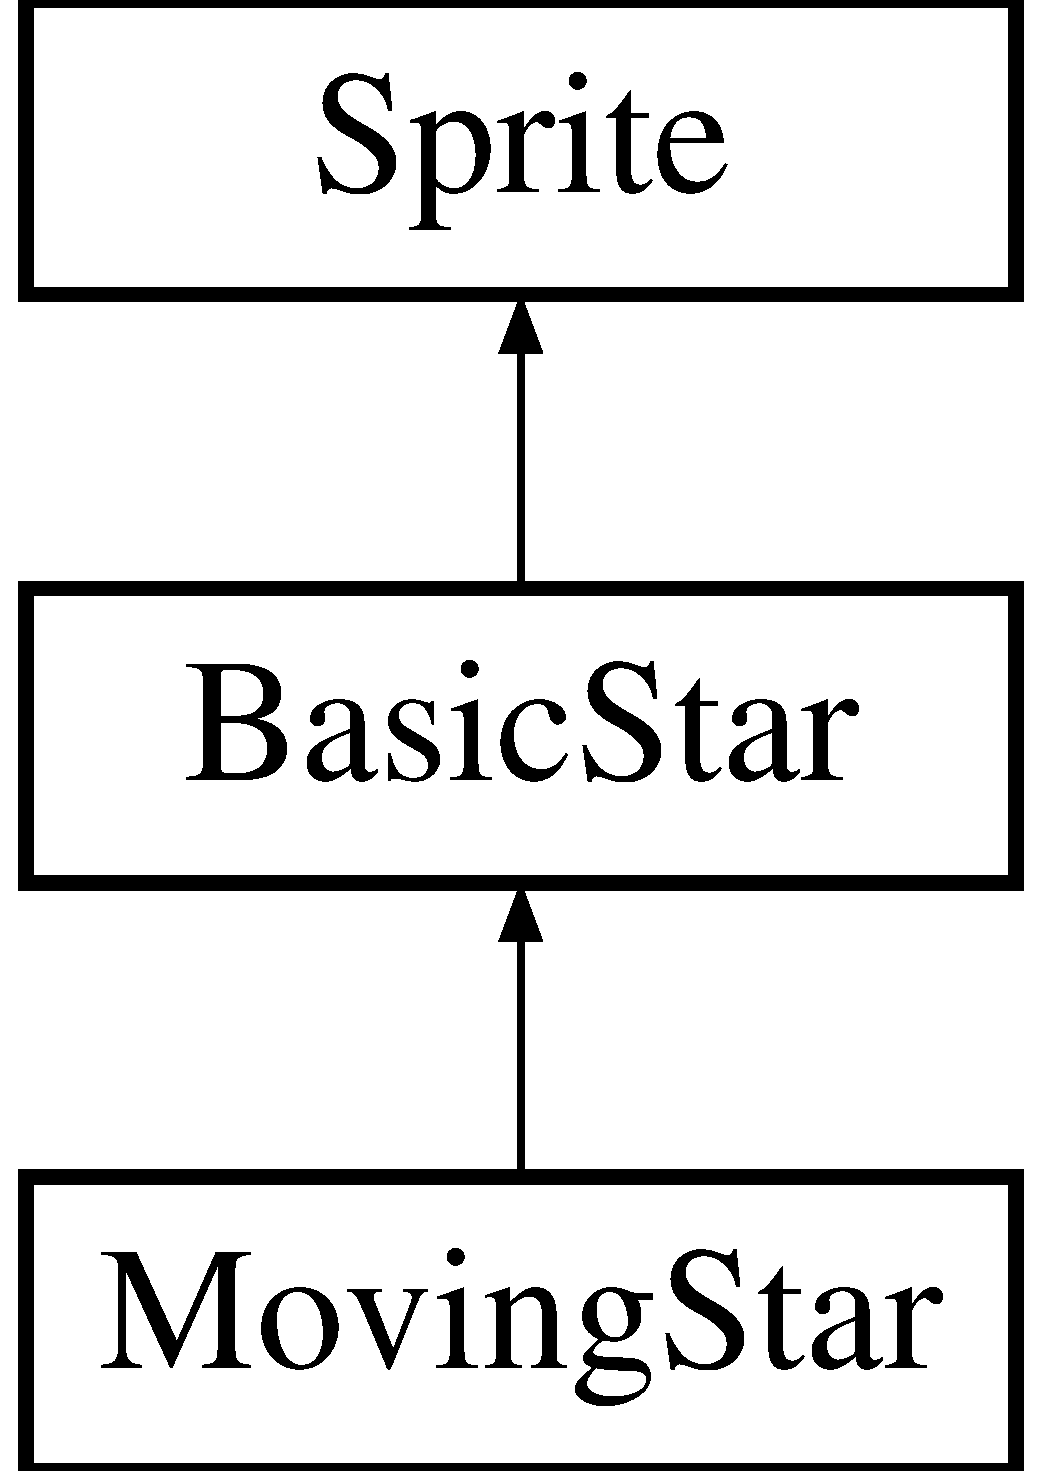
\includegraphics[height=2.000000cm]{classBasicStar}
\end{center}
\end{figure}
\subsection*{Public Member Functions}
\begin{DoxyCompactItemize}
\item 
\hyperlink{classBasicStar_a7cda590583a4a67c057487c7fc61281b}{Basic\-Star} (short \hyperlink{classSprite_afca2c03aad9d2526427470688ae76439}{y}, int edge\-\_\-coord)
\begin{DoxyCompactList}\small\item\em Constructor. \end{DoxyCompactList}\item 
\hyperlink{classBasicStar_a6ac994000481a4e155a16c4f96f9e17b}{$\sim$\-Basic\-Star} ()
\begin{DoxyCompactList}\small\item\em Destructor. \end{DoxyCompactList}\end{DoxyCompactItemize}
\subsection*{Private Member Functions}
\begin{DoxyCompactItemize}
\item 
void \hyperlink{classBasicStar_ad978bef7512c6f5df863049d90cf0da8}{randomize\-Spawn} (int edge\-\_\-coord)
\begin{DoxyCompactList}\small\item\em Set the enemy's x to a random number. \end{DoxyCompactList}\end{DoxyCompactItemize}
\subsection*{Additional Inherited Members}


\subsection{Detailed Description}
The most basic type of star, cannot move. 

\subsection{Constructor \& Destructor Documentation}
\hypertarget{classBasicStar_a7cda590583a4a67c057487c7fc61281b}{\index{Basic\-Star@{Basic\-Star}!Basic\-Star@{Basic\-Star}}
\index{Basic\-Star@{Basic\-Star}!BasicStar@{Basic\-Star}}
\subsubsection[{Basic\-Star}]{\setlength{\rightskip}{0pt plus 5cm}Basic\-Star\-::\-Basic\-Star (
\begin{DoxyParamCaption}
\item[{short}]{y, }
\item[{int}]{edge\-\_\-coord}
\end{DoxyParamCaption}
)}}\label{classBasicStar_a7cda590583a4a67c057487c7fc61281b}


Constructor. 


\begin{DoxyParams}{Parameters}
{\em y} & position of last \hyperlink{classBasicStar}{Basic\-Star} \\
\hline
{\em edge\-\_\-coord} & how many pixels we need to move to escape the screen \\
\hline
\end{DoxyParams}
\hypertarget{classBasicStar_a6ac994000481a4e155a16c4f96f9e17b}{\index{Basic\-Star@{Basic\-Star}!$\sim$\-Basic\-Star@{$\sim$\-Basic\-Star}}
\index{$\sim$\-Basic\-Star@{$\sim$\-Basic\-Star}!BasicStar@{Basic\-Star}}
\subsubsection[{$\sim$\-Basic\-Star}]{\setlength{\rightskip}{0pt plus 5cm}Basic\-Star\-::$\sim$\-Basic\-Star (
\begin{DoxyParamCaption}
{}
\end{DoxyParamCaption}
)}}\label{classBasicStar_a6ac994000481a4e155a16c4f96f9e17b}


Destructor. 



\subsection{Member Function Documentation}
\hypertarget{classBasicStar_ad978bef7512c6f5df863049d90cf0da8}{\index{Basic\-Star@{Basic\-Star}!randomize\-Spawn@{randomize\-Spawn}}
\index{randomize\-Spawn@{randomize\-Spawn}!BasicStar@{Basic\-Star}}
\subsubsection[{randomize\-Spawn}]{\setlength{\rightskip}{0pt plus 5cm}void Basic\-Star\-::randomize\-Spawn (
\begin{DoxyParamCaption}
\item[{int}]{edge\-\_\-coord}
\end{DoxyParamCaption}
)\hspace{0.3cm}{\ttfamily [private]}}}\label{classBasicStar_ad978bef7512c6f5df863049d90cf0da8}


Set the enemy's x to a random number. 


\begin{DoxyParams}{Parameters}
{\em edge\-\_\-coord} & how many pixels we need to move to escape the screen \\
\hline
\end{DoxyParams}


The documentation for this class was generated from the following files\-:\begin{DoxyCompactItemize}
\item 
src/\hyperlink{BasicStar_8hh}{Basic\-Star.\-hh}\item 
src/\hyperlink{BasicStar_8cc}{Basic\-Star.\-cc}\end{DoxyCompactItemize}

\hypertarget{classGame}{\section{Game Class Reference}
\label{classGame}\index{Game@{Game}}
}


Main game class.  




{\ttfamily \#include $<$Game.\-hh$>$}

\subsection*{Public Member Functions}
\begin{DoxyCompactItemize}
\item 
\hyperlink{classGame_ad59df6562a58a614fda24622d3715b65}{Game} ()
\begin{DoxyCompactList}\small\item\em Constructor. \end{DoxyCompactList}\item 
\hyperlink{classGame_ae3d112ca6e0e55150d2fdbc704474530}{$\sim$\-Game} ()
\begin{DoxyCompactList}\small\item\em Destructor. \end{DoxyCompactList}\item 
int \hyperlink{classGame_a99fb161fbbe87d25a8b73265a0611e58}{run} ()
\begin{DoxyCompactList}\small\item\em The game's main loop. \end{DoxyCompactList}\end{DoxyCompactItemize}
\subsection*{Private Member Functions}
\begin{DoxyCompactItemize}
\item 
int \hyperlink{classGame_aed445257fc658cf0d8be31c174c0e42e}{add\-Enemies} (std\-::list$<$ \hyperlink{classBasicEnemy}{Basic\-Enemy} $>$ \&enemies)
\begin{DoxyCompactList}\small\item\em Add enemies until they fill up the screen. \end{DoxyCompactList}\item 
\hyperlink{classGame_aa79443880de5f26387c2a1c70c8c1aae}{Game} (const \hyperlink{classGame}{Game} \&)
\begin{DoxyCompactList}\small\item\em Disabled copy constructor. \end{DoxyCompactList}\item 
void \hyperlink{classGame_a33d46168923cdeca0d97553fc47e050e}{operator=} (const \hyperlink{classGame}{Game} \&)
\begin{DoxyCompactList}\small\item\em Disabled copy constructor. \end{DoxyCompactList}\end{DoxyCompactItemize}
\subsection*{Private Attributes}
\begin{DoxyCompactItemize}
\item 
\hyperlink{classGraphicsEngine}{Graphics\-Engine} $\ast$ \hyperlink{classGame_ac96e150f595f287b0e32ff2ad15ef663}{graphics\-\_\-}
\begin{DoxyCompactList}\small\item\em Instance for managing graphics. \end{DoxyCompactList}\end{DoxyCompactItemize}


\subsection{Detailed Description}
Main game class. 

\hyperlink{classGame}{Game} is the main class, which acts as the core of the application It's role is glue the other projects together in a structured way without doing any work by itself 

\subsection{Constructor \& Destructor Documentation}
\hypertarget{classGame_ad59df6562a58a614fda24622d3715b65}{\index{Game@{Game}!Game@{Game}}
\index{Game@{Game}!Game@{Game}}
\subsubsection[{Game}]{\setlength{\rightskip}{0pt plus 5cm}Game\-::\-Game (
\begin{DoxyParamCaption}
{}
\end{DoxyParamCaption}
)}}\label{classGame_ad59df6562a58a614fda24622d3715b65}


Constructor. 

\hypertarget{classGame_ae3d112ca6e0e55150d2fdbc704474530}{\index{Game@{Game}!$\sim$\-Game@{$\sim$\-Game}}
\index{$\sim$\-Game@{$\sim$\-Game}!Game@{Game}}
\subsubsection[{$\sim$\-Game}]{\setlength{\rightskip}{0pt plus 5cm}Game\-::$\sim$\-Game (
\begin{DoxyParamCaption}
{}
\end{DoxyParamCaption}
)}}\label{classGame_ae3d112ca6e0e55150d2fdbc704474530}


Destructor. 

\hypertarget{classGame_aa79443880de5f26387c2a1c70c8c1aae}{\index{Game@{Game}!Game@{Game}}
\index{Game@{Game}!Game@{Game}}
\subsubsection[{Game}]{\setlength{\rightskip}{0pt plus 5cm}Game\-::\-Game (
\begin{DoxyParamCaption}
\item[{const {\bf Game} \&}]{}
\end{DoxyParamCaption}
)\hspace{0.3cm}{\ttfamily [private]}}}\label{classGame_aa79443880de5f26387c2a1c70c8c1aae}


Disabled copy constructor. 



\subsection{Member Function Documentation}
\hypertarget{classGame_aed445257fc658cf0d8be31c174c0e42e}{\index{Game@{Game}!add\-Enemies@{add\-Enemies}}
\index{add\-Enemies@{add\-Enemies}!Game@{Game}}
\subsubsection[{add\-Enemies}]{\setlength{\rightskip}{0pt plus 5cm}int Game\-::add\-Enemies (
\begin{DoxyParamCaption}
\item[{std\-::list$<$ {\bf Basic\-Enemy} $>$ \&}]{enemies}
\end{DoxyParamCaption}
)\hspace{0.3cm}{\ttfamily [private]}}}\label{classGame_aed445257fc658cf0d8be31c174c0e42e}


Add enemies until they fill up the screen. 


\begin{DoxyParams}{Parameters}
{\em enemies} & list of enemies in \hyperlink{classGame_a99fb161fbbe87d25a8b73265a0611e58}{run()}-\/function \\
\hline
\end{DoxyParams}
\hypertarget{classGame_a33d46168923cdeca0d97553fc47e050e}{\index{Game@{Game}!operator=@{operator=}}
\index{operator=@{operator=}!Game@{Game}}
\subsubsection[{operator=}]{\setlength{\rightskip}{0pt plus 5cm}void Game\-::operator= (
\begin{DoxyParamCaption}
\item[{const {\bf Game} \&}]{}
\end{DoxyParamCaption}
)\hspace{0.3cm}{\ttfamily [private]}}}\label{classGame_a33d46168923cdeca0d97553fc47e050e}


Disabled copy constructor. 

\hypertarget{classGame_a99fb161fbbe87d25a8b73265a0611e58}{\index{Game@{Game}!run@{run}}
\index{run@{run}!Game@{Game}}
\subsubsection[{run}]{\setlength{\rightskip}{0pt plus 5cm}int Game\-::run (
\begin{DoxyParamCaption}
{}
\end{DoxyParamCaption}
)}}\label{classGame_a99fb161fbbe87d25a8b73265a0611e58}


The game's main loop. 

\begin{DoxyReturn}{Returns}
0 on success 
\end{DoxyReturn}


\subsection{Member Data Documentation}
\hypertarget{classGame_ac96e150f595f287b0e32ff2ad15ef663}{\index{Game@{Game}!graphics\-\_\-@{graphics\-\_\-}}
\index{graphics\-\_\-@{graphics\-\_\-}!Game@{Game}}
\subsubsection[{graphics\-\_\-}]{\setlength{\rightskip}{0pt plus 5cm}{\bf Graphics\-Engine}$\ast$ Game\-::graphics\-\_\-\hspace{0.3cm}{\ttfamily [private]}}}\label{classGame_ac96e150f595f287b0e32ff2ad15ef663}


Instance for managing graphics. 



The documentation for this class was generated from the following files\-:\begin{DoxyCompactItemize}
\item 
src/\hyperlink{Game_8hh}{Game.\-hh}\item 
src/\hyperlink{Game_8cc}{Game.\-cc}\end{DoxyCompactItemize}

\hypertarget{classGraphicsEngine}{\section{Graphics\-Engine Class Reference}
\label{classGraphicsEngine}\index{Graphics\-Engine@{Graphics\-Engine}}
}


Class for managing graphics and events.  




{\ttfamily \#include $<$Graphics\-Engine.\-hh$>$}

\subsection*{Public Member Functions}
\begin{DoxyCompactItemize}
\item 
\hyperlink{classGraphicsEngine_afb12af77895e3bbb57e6d46a36ba3974}{Graphics\-Engine} (const std\-::string \&title, const unsigned \hyperlink{classGraphicsEngine_a7598618ef7de1ba7813e41471938f2c1}{screen\-\_\-width}, const unsigned \hyperlink{classGraphicsEngine_af7d7440d76fda157dae03aabc9388a83}{screen\-\_\-height}, const unsigned screen\-\_\-bpp, const unsigned frame\-\_\-rate)
\begin{DoxyCompactList}\small\item\em Contructor. \end{DoxyCompactList}\item 
\hyperlink{classGraphicsEngine_ab67afeefbc9f1c284f6ce310c31ae8f6}{$\sim$\-Graphics\-Engine} ()
\begin{DoxyCompactList}\small\item\em Destructor. \end{DoxyCompactList}\item 
bool \hyperlink{classGraphicsEngine_a2588ff40788701709e97107100e0a8f3}{load\-Image} (const std\-::string \&filename)
\begin{DoxyCompactList}\small\item\em Loads and image from the disk into the R\-A\-M. \end{DoxyCompactList}\item 
std\-::string \hyperlink{classGraphicsEngine_a0141ef903d368eedea2aaf6e47001efa}{get\-Last\-Error} () const 
\begin{DoxyCompactList}\small\item\em returns a string describing last error that occurred \end{DoxyCompactList}\item 
bool \hyperlink{classGraphicsEngine_a47be08aa9a766dce3b32b6814fb5b6ed}{draw\-Image} (const std\-::string \&image, \hyperlink{GraphicsEngine_8hh_a9a150f1ad43ec7de65cfe698cdae8bee}{rect\-\_\-t} $\ast$srcrect, \hyperlink{GraphicsEngine_8hh_a9a150f1ad43ec7de65cfe698cdae8bee}{rect\-\_\-t} $\ast$dstrect)
\begin{DoxyCompactList}\small\item\em Draw an image to the game screen. \end{DoxyCompactList}\item 
void \hyperlink{classGraphicsEngine_a82d4584abba7fd03c321a3e418964cac}{draw\-Text} (const std\-::string \&text, unsigned x, unsigned y)
\begin{DoxyCompactList}\small\item\em Draw some text at the given location. \end{DoxyCompactList}\item 
bool \hyperlink{classGraphicsEngine_aeadd04c5518ef05b039241cbb7d09b59}{update\-Screen} ()
\begin{DoxyCompactList}\small\item\em Flushes the screen so it's visible to the user. \end{DoxyCompactList}\item 
bool \hyperlink{classGraphicsEngine_acdcf6935481bebcc5f45e7fd18dcf016}{get\-Event} (\hyperlink{GraphicsEngine_8hh_a2fb9b58e4e5f14f40af8b4a1425841f8}{event\-\_\-t} \&event) const 
\begin{DoxyCompactList}\small\item\em Non-\/blocking function to check event depending on user input. \end{DoxyCompactList}\item 
void \hyperlink{classGraphicsEngine_a4fe915afad2a770445f34ad1f597474a}{wait\-For\-Keypress} () const 
\begin{DoxyCompactList}\small\item\em Waits until a key is pressed. \end{DoxyCompactList}\item 
unsigned \hyperlink{classGraphicsEngine_a7598618ef7de1ba7813e41471938f2c1}{screen\-\_\-width} () const 
\begin{DoxyCompactList}\small\item\em Returns width of game screen. \end{DoxyCompactList}\item 
unsigned \hyperlink{classGraphicsEngine_af7d7440d76fda157dae03aabc9388a83}{screen\-\_\-height} () const 
\begin{DoxyCompactList}\small\item\em Returns height of game screen. \end{DoxyCompactList}\end{DoxyCompactItemize}
\subsection*{Private Member Functions}
\begin{DoxyCompactItemize}
\item 
\hyperlink{classGraphicsEngine_a6b6f92b943fc986f687b4d7797f2fa2a}{Graphics\-Engine} (const \hyperlink{classGraphicsEngine}{Graphics\-Engine} \&)
\begin{DoxyCompactList}\small\item\em Copy constructor (D\-O N\-O\-T U\-S\-E) \end{DoxyCompactList}\item 
void \hyperlink{classGraphicsEngine_af942976c09aac7332c8425b6a0130688}{operator=} (const \hyperlink{classGraphicsEngine}{Graphics\-Engine} \&)
\begin{DoxyCompactList}\small\item\em Copy constructor (D\-O N\-O\-T U\-S\-E) \end{DoxyCompactList}\end{DoxyCompactItemize}
\subsection*{Private Attributes}
\begin{DoxyCompactItemize}
\item 
const std\-::string \hyperlink{classGraphicsEngine_afc40023b292929b8b8e53c58b7e8f574}{T\-I\-T\-L\-E}
\begin{DoxyCompactList}\small\item\em Title to display on the game's status bar. \end{DoxyCompactList}\item 
const unsigned \hyperlink{classGraphicsEngine_ac243d365dcf3e8a14f8ff1a838479429}{S\-C\-R\-E\-E\-N\-\_\-\-W\-I\-D\-T\-H}
\begin{DoxyCompactList}\small\item\em Width of the game screen. \end{DoxyCompactList}\item 
const unsigned \hyperlink{classGraphicsEngine_a22ccc86caef4284dcf8600ef846e3897}{S\-C\-R\-E\-E\-N\-\_\-\-H\-E\-I\-G\-H\-T}
\begin{DoxyCompactList}\small\item\em Height of the game screen. \end{DoxyCompactList}\item 
const unsigned \hyperlink{classGraphicsEngine_a3ff7024552553e73dd9edaef063284e0}{S\-C\-R\-E\-E\-N\-\_\-\-B\-P\-P}
\begin{DoxyCompactList}\small\item\em Screen bits per pixel (color) \end{DoxyCompactList}\item 
const unsigned short \hyperlink{classGraphicsEngine_a488d694ad4eea9bbbe68fc4d98cde8bf}{F\-R\-A\-M\-E\-\_\-\-R\-A\-T\-E}
\begin{DoxyCompactList}\small\item\em Screen frames per second. \end{DoxyCompactList}\item 
std\-::map$<$ std\-::string, \\*
S\-D\-L\-\_\-\-Surface $\ast$ $>$ \hyperlink{classGraphicsEngine_a5058ffe9d65389df4207db6be00ac889}{images\-\_\-}
\begin{DoxyCompactList}\small\item\em Map of filename and image we have loaded from disk. \end{DoxyCompactList}\item 
size\-\_\-t \hyperlink{classGraphicsEngine_a03732739efdf1f24a3bda1a202b6b866}{time\-\_\-of\-\_\-last\-\_\-refresh\-\_\-}
\begin{DoxyCompactList}\small\item\em The time \hyperlink{classGraphicsEngine_aeadd04c5518ef05b039241cbb7d09b59}{update\-Screen()} last was called. \end{DoxyCompactList}\item 
S\-D\-L\-\_\-\-Surface $\ast$ \hyperlink{classGraphicsEngine_a4d89c081a99c7512a070c9cb77809322}{screen\-\_\-}
\begin{DoxyCompactList}\small\item\em The game screen. \end{DoxyCompactList}\item 
T\-T\-F\-\_\-\-Font $\ast$ \hyperlink{classGraphicsEngine_aea94592fe91edfb3983a0ee088f2888b}{font\-\_\-}
\begin{DoxyCompactList}\small\item\em Font to use. \end{DoxyCompactList}\end{DoxyCompactItemize}


\subsection{Detailed Description}
Class for managing graphics and events. 

\hyperlink{classGraphicsEngine}{Graphics\-Engine} handles all input from the user and handles all drawing of images on the screen. Only one \hyperlink{classGraphicsEngine}{Graphics\-Engine} can be active at one time 

\subsection{Constructor \& Destructor Documentation}
\hypertarget{classGraphicsEngine_afb12af77895e3bbb57e6d46a36ba3974}{\index{Graphics\-Engine@{Graphics\-Engine}!Graphics\-Engine@{Graphics\-Engine}}
\index{Graphics\-Engine@{Graphics\-Engine}!GraphicsEngine@{Graphics\-Engine}}
\subsubsection[{Graphics\-Engine}]{\setlength{\rightskip}{0pt plus 5cm}Graphics\-Engine\-::\-Graphics\-Engine (
\begin{DoxyParamCaption}
\item[{const std\-::string \&}]{title, }
\item[{const unsigned}]{screen\-\_\-width, }
\item[{const unsigned}]{screen\-\_\-height, }
\item[{const unsigned}]{screen\-\_\-bpp, }
\item[{const unsigned}]{frame\-\_\-rate}
\end{DoxyParamCaption}
)}}\label{classGraphicsEngine_afb12af77895e3bbb57e6d46a36ba3974}


Contructor. 


\begin{DoxyParams}{Parameters}
{\em title} & The title that will be seen on the titlebar \\
\hline
{\em screen\-\_\-width} & Size of game screen's width \\
\hline
{\em screen\-\_\-height} & Size of the game screen's height \\
\hline
{\em screen\-\_\-bpp} & The amount of bits per pixel (color) \\
\hline
{\em frame\-\_\-rate} & The frames per second we want to display \\
\hline
\end{DoxyParams}
\hypertarget{classGraphicsEngine_ab67afeefbc9f1c284f6ce310c31ae8f6}{\index{Graphics\-Engine@{Graphics\-Engine}!$\sim$\-Graphics\-Engine@{$\sim$\-Graphics\-Engine}}
\index{$\sim$\-Graphics\-Engine@{$\sim$\-Graphics\-Engine}!GraphicsEngine@{Graphics\-Engine}}
\subsubsection[{$\sim$\-Graphics\-Engine}]{\setlength{\rightskip}{0pt plus 5cm}Graphics\-Engine\-::$\sim$\-Graphics\-Engine (
\begin{DoxyParamCaption}
{}
\end{DoxyParamCaption}
)}}\label{classGraphicsEngine_ab67afeefbc9f1c284f6ce310c31ae8f6}


Destructor. 

\hypertarget{classGraphicsEngine_a6b6f92b943fc986f687b4d7797f2fa2a}{\index{Graphics\-Engine@{Graphics\-Engine}!Graphics\-Engine@{Graphics\-Engine}}
\index{Graphics\-Engine@{Graphics\-Engine}!GraphicsEngine@{Graphics\-Engine}}
\subsubsection[{Graphics\-Engine}]{\setlength{\rightskip}{0pt plus 5cm}Graphics\-Engine\-::\-Graphics\-Engine (
\begin{DoxyParamCaption}
\item[{const {\bf Graphics\-Engine} \&}]{}
\end{DoxyParamCaption}
)\hspace{0.3cm}{\ttfamily [private]}}}\label{classGraphicsEngine_a6b6f92b943fc986f687b4d7797f2fa2a}


Copy constructor (D\-O N\-O\-T U\-S\-E) 



\subsection{Member Function Documentation}
\hypertarget{classGraphicsEngine_a47be08aa9a766dce3b32b6814fb5b6ed}{\index{Graphics\-Engine@{Graphics\-Engine}!draw\-Image@{draw\-Image}}
\index{draw\-Image@{draw\-Image}!GraphicsEngine@{Graphics\-Engine}}
\subsubsection[{draw\-Image}]{\setlength{\rightskip}{0pt plus 5cm}bool Graphics\-Engine\-::draw\-Image (
\begin{DoxyParamCaption}
\item[{const std\-::string \&}]{image, }
\item[{{\bf rect\-\_\-t} $\ast$}]{srcrect, }
\item[{{\bf rect\-\_\-t} $\ast$}]{dstrect}
\end{DoxyParamCaption}
)}}\label{classGraphicsEngine_a47be08aa9a766dce3b32b6814fb5b6ed}


Draw an image to the game screen. 


\begin{DoxyParams}{Parameters}
{\em image} & filename of image to draw \\
\hline
{\em srcrect} & rectangle of image to draw from \\
\hline
{\em dstrect} & part to screen to draw to \\
\hline
\end{DoxyParams}
\begin{DoxyReturn}{Returns}
true on success 
\end{DoxyReturn}
\hypertarget{classGraphicsEngine_a82d4584abba7fd03c321a3e418964cac}{\index{Graphics\-Engine@{Graphics\-Engine}!draw\-Text@{draw\-Text}}
\index{draw\-Text@{draw\-Text}!GraphicsEngine@{Graphics\-Engine}}
\subsubsection[{draw\-Text}]{\setlength{\rightskip}{0pt plus 5cm}void Graphics\-Engine\-::draw\-Text (
\begin{DoxyParamCaption}
\item[{const std\-::string \&}]{text, }
\item[{unsigned}]{x, }
\item[{unsigned}]{y}
\end{DoxyParamCaption}
)}}\label{classGraphicsEngine_a82d4584abba7fd03c321a3e418964cac}


Draw some text at the given location. 


\begin{DoxyParams}{Parameters}
{\em text} & text to draw \\
\hline
{\em x} & the center on the x-\/axis where we will draw \\
\hline
{\em y} & the center on the y-\/axis where we will draw \\
\hline
\end{DoxyParams}
\hypertarget{classGraphicsEngine_acdcf6935481bebcc5f45e7fd18dcf016}{\index{Graphics\-Engine@{Graphics\-Engine}!get\-Event@{get\-Event}}
\index{get\-Event@{get\-Event}!GraphicsEngine@{Graphics\-Engine}}
\subsubsection[{get\-Event}]{\setlength{\rightskip}{0pt plus 5cm}bool Graphics\-Engine\-::get\-Event (
\begin{DoxyParamCaption}
\item[{{\bf event\-\_\-t} \&}]{event}
\end{DoxyParamCaption}
) const}}\label{classGraphicsEngine_acdcf6935481bebcc5f45e7fd18dcf016}


Non-\/blocking function to check event depending on user input. 


\begin{DoxyParams}{Parameters}
{\em event} & The event received from user \\
\hline
\end{DoxyParams}
\begin{DoxyReturn}{Returns}
true if there are more pending events 
\end{DoxyReturn}
\hypertarget{classGraphicsEngine_a0141ef903d368eedea2aaf6e47001efa}{\index{Graphics\-Engine@{Graphics\-Engine}!get\-Last\-Error@{get\-Last\-Error}}
\index{get\-Last\-Error@{get\-Last\-Error}!GraphicsEngine@{Graphics\-Engine}}
\subsubsection[{get\-Last\-Error}]{\setlength{\rightskip}{0pt plus 5cm}string Graphics\-Engine\-::get\-Last\-Error (
\begin{DoxyParamCaption}
{}
\end{DoxyParamCaption}
) const}}\label{classGraphicsEngine_a0141ef903d368eedea2aaf6e47001efa}


returns a string describing last error that occurred 

\hypertarget{classGraphicsEngine_a2588ff40788701709e97107100e0a8f3}{\index{Graphics\-Engine@{Graphics\-Engine}!load\-Image@{load\-Image}}
\index{load\-Image@{load\-Image}!GraphicsEngine@{Graphics\-Engine}}
\subsubsection[{load\-Image}]{\setlength{\rightskip}{0pt plus 5cm}bool Graphics\-Engine\-::load\-Image (
\begin{DoxyParamCaption}
\item[{const std\-::string \&}]{filename}
\end{DoxyParamCaption}
)}}\label{classGraphicsEngine_a2588ff40788701709e97107100e0a8f3}


Loads and image from the disk into the R\-A\-M. 


\begin{DoxyParams}{Parameters}
{\em filename} & Name of the image file inside graphics/ folder (example\-: to load graphics/player.\-png, filename should be \char`\"{}player\char`\"{}) \\
\hline
\end{DoxyParams}
\begin{DoxyReturn}{Returns}
true on success 
\end{DoxyReturn}
\hypertarget{classGraphicsEngine_af942976c09aac7332c8425b6a0130688}{\index{Graphics\-Engine@{Graphics\-Engine}!operator=@{operator=}}
\index{operator=@{operator=}!GraphicsEngine@{Graphics\-Engine}}
\subsubsection[{operator=}]{\setlength{\rightskip}{0pt plus 5cm}void Graphics\-Engine\-::operator= (
\begin{DoxyParamCaption}
\item[{const {\bf Graphics\-Engine} \&}]{}
\end{DoxyParamCaption}
)\hspace{0.3cm}{\ttfamily [private]}}}\label{classGraphicsEngine_af942976c09aac7332c8425b6a0130688}


Copy constructor (D\-O N\-O\-T U\-S\-E) 

\hypertarget{classGraphicsEngine_af7d7440d76fda157dae03aabc9388a83}{\index{Graphics\-Engine@{Graphics\-Engine}!screen\-\_\-height@{screen\-\_\-height}}
\index{screen\-\_\-height@{screen\-\_\-height}!GraphicsEngine@{Graphics\-Engine}}
\subsubsection[{screen\-\_\-height}]{\setlength{\rightskip}{0pt plus 5cm}unsigned Graphics\-Engine\-::screen\-\_\-height (
\begin{DoxyParamCaption}
{}
\end{DoxyParamCaption}
) const}}\label{classGraphicsEngine_af7d7440d76fda157dae03aabc9388a83}


Returns height of game screen. 

\hypertarget{classGraphicsEngine_a7598618ef7de1ba7813e41471938f2c1}{\index{Graphics\-Engine@{Graphics\-Engine}!screen\-\_\-width@{screen\-\_\-width}}
\index{screen\-\_\-width@{screen\-\_\-width}!GraphicsEngine@{Graphics\-Engine}}
\subsubsection[{screen\-\_\-width}]{\setlength{\rightskip}{0pt plus 5cm}unsigned Graphics\-Engine\-::screen\-\_\-width (
\begin{DoxyParamCaption}
{}
\end{DoxyParamCaption}
) const}}\label{classGraphicsEngine_a7598618ef7de1ba7813e41471938f2c1}


Returns width of game screen. 

\hypertarget{classGraphicsEngine_aeadd04c5518ef05b039241cbb7d09b59}{\index{Graphics\-Engine@{Graphics\-Engine}!update\-Screen@{update\-Screen}}
\index{update\-Screen@{update\-Screen}!GraphicsEngine@{Graphics\-Engine}}
\subsubsection[{update\-Screen}]{\setlength{\rightskip}{0pt plus 5cm}bool Graphics\-Engine\-::update\-Screen (
\begin{DoxyParamCaption}
{}
\end{DoxyParamCaption}
)}}\label{classGraphicsEngine_aeadd04c5518ef05b039241cbb7d09b59}


Flushes the screen so it's visible to the user. 

\begin{DoxyReturn}{Returns}
true on success 
\end{DoxyReturn}
\hypertarget{classGraphicsEngine_a4fe915afad2a770445f34ad1f597474a}{\index{Graphics\-Engine@{Graphics\-Engine}!wait\-For\-Keypress@{wait\-For\-Keypress}}
\index{wait\-For\-Keypress@{wait\-For\-Keypress}!GraphicsEngine@{Graphics\-Engine}}
\subsubsection[{wait\-For\-Keypress}]{\setlength{\rightskip}{0pt plus 5cm}void Graphics\-Engine\-::wait\-For\-Keypress (
\begin{DoxyParamCaption}
{}
\end{DoxyParamCaption}
) const}}\label{classGraphicsEngine_a4fe915afad2a770445f34ad1f597474a}


Waits until a key is pressed. 



\subsection{Member Data Documentation}
\hypertarget{classGraphicsEngine_aea94592fe91edfb3983a0ee088f2888b}{\index{Graphics\-Engine@{Graphics\-Engine}!font\-\_\-@{font\-\_\-}}
\index{font\-\_\-@{font\-\_\-}!GraphicsEngine@{Graphics\-Engine}}
\subsubsection[{font\-\_\-}]{\setlength{\rightskip}{0pt plus 5cm}T\-T\-F\-\_\-\-Font$\ast$ Graphics\-Engine\-::font\-\_\-\hspace{0.3cm}{\ttfamily [private]}}}\label{classGraphicsEngine_aea94592fe91edfb3983a0ee088f2888b}


Font to use. 

\hypertarget{classGraphicsEngine_a488d694ad4eea9bbbe68fc4d98cde8bf}{\index{Graphics\-Engine@{Graphics\-Engine}!F\-R\-A\-M\-E\-\_\-\-R\-A\-T\-E@{F\-R\-A\-M\-E\-\_\-\-R\-A\-T\-E}}
\index{F\-R\-A\-M\-E\-\_\-\-R\-A\-T\-E@{F\-R\-A\-M\-E\-\_\-\-R\-A\-T\-E}!GraphicsEngine@{Graphics\-Engine}}
\subsubsection[{F\-R\-A\-M\-E\-\_\-\-R\-A\-T\-E}]{\setlength{\rightskip}{0pt plus 5cm}const unsigned short Graphics\-Engine\-::\-F\-R\-A\-M\-E\-\_\-\-R\-A\-T\-E\hspace{0.3cm}{\ttfamily [private]}}}\label{classGraphicsEngine_a488d694ad4eea9bbbe68fc4d98cde8bf}


Screen frames per second. 

\hypertarget{classGraphicsEngine_a5058ffe9d65389df4207db6be00ac889}{\index{Graphics\-Engine@{Graphics\-Engine}!images\-\_\-@{images\-\_\-}}
\index{images\-\_\-@{images\-\_\-}!GraphicsEngine@{Graphics\-Engine}}
\subsubsection[{images\-\_\-}]{\setlength{\rightskip}{0pt plus 5cm}std\-::map$<$std\-::string, S\-D\-L\-\_\-\-Surface $\ast$$>$ Graphics\-Engine\-::images\-\_\-\hspace{0.3cm}{\ttfamily [private]}}}\label{classGraphicsEngine_a5058ffe9d65389df4207db6be00ac889}


Map of filename and image we have loaded from disk. 

\hypertarget{classGraphicsEngine_a4d89c081a99c7512a070c9cb77809322}{\index{Graphics\-Engine@{Graphics\-Engine}!screen\-\_\-@{screen\-\_\-}}
\index{screen\-\_\-@{screen\-\_\-}!GraphicsEngine@{Graphics\-Engine}}
\subsubsection[{screen\-\_\-}]{\setlength{\rightskip}{0pt plus 5cm}S\-D\-L\-\_\-\-Surface$\ast$ Graphics\-Engine\-::screen\-\_\-\hspace{0.3cm}{\ttfamily [private]}}}\label{classGraphicsEngine_a4d89c081a99c7512a070c9cb77809322}


The game screen. 

\hypertarget{classGraphicsEngine_a3ff7024552553e73dd9edaef063284e0}{\index{Graphics\-Engine@{Graphics\-Engine}!S\-C\-R\-E\-E\-N\-\_\-\-B\-P\-P@{S\-C\-R\-E\-E\-N\-\_\-\-B\-P\-P}}
\index{S\-C\-R\-E\-E\-N\-\_\-\-B\-P\-P@{S\-C\-R\-E\-E\-N\-\_\-\-B\-P\-P}!GraphicsEngine@{Graphics\-Engine}}
\subsubsection[{S\-C\-R\-E\-E\-N\-\_\-\-B\-P\-P}]{\setlength{\rightskip}{0pt plus 5cm}const unsigned Graphics\-Engine\-::\-S\-C\-R\-E\-E\-N\-\_\-\-B\-P\-P\hspace{0.3cm}{\ttfamily [private]}}}\label{classGraphicsEngine_a3ff7024552553e73dd9edaef063284e0}


Screen bits per pixel (color) 

\hypertarget{classGraphicsEngine_a22ccc86caef4284dcf8600ef846e3897}{\index{Graphics\-Engine@{Graphics\-Engine}!S\-C\-R\-E\-E\-N\-\_\-\-H\-E\-I\-G\-H\-T@{S\-C\-R\-E\-E\-N\-\_\-\-H\-E\-I\-G\-H\-T}}
\index{S\-C\-R\-E\-E\-N\-\_\-\-H\-E\-I\-G\-H\-T@{S\-C\-R\-E\-E\-N\-\_\-\-H\-E\-I\-G\-H\-T}!GraphicsEngine@{Graphics\-Engine}}
\subsubsection[{S\-C\-R\-E\-E\-N\-\_\-\-H\-E\-I\-G\-H\-T}]{\setlength{\rightskip}{0pt plus 5cm}const unsigned Graphics\-Engine\-::\-S\-C\-R\-E\-E\-N\-\_\-\-H\-E\-I\-G\-H\-T\hspace{0.3cm}{\ttfamily [private]}}}\label{classGraphicsEngine_a22ccc86caef4284dcf8600ef846e3897}


Height of the game screen. 

\hypertarget{classGraphicsEngine_ac243d365dcf3e8a14f8ff1a838479429}{\index{Graphics\-Engine@{Graphics\-Engine}!S\-C\-R\-E\-E\-N\-\_\-\-W\-I\-D\-T\-H@{S\-C\-R\-E\-E\-N\-\_\-\-W\-I\-D\-T\-H}}
\index{S\-C\-R\-E\-E\-N\-\_\-\-W\-I\-D\-T\-H@{S\-C\-R\-E\-E\-N\-\_\-\-W\-I\-D\-T\-H}!GraphicsEngine@{Graphics\-Engine}}
\subsubsection[{S\-C\-R\-E\-E\-N\-\_\-\-W\-I\-D\-T\-H}]{\setlength{\rightskip}{0pt plus 5cm}const unsigned Graphics\-Engine\-::\-S\-C\-R\-E\-E\-N\-\_\-\-W\-I\-D\-T\-H\hspace{0.3cm}{\ttfamily [private]}}}\label{classGraphicsEngine_ac243d365dcf3e8a14f8ff1a838479429}


Width of the game screen. 

\hypertarget{classGraphicsEngine_a03732739efdf1f24a3bda1a202b6b866}{\index{Graphics\-Engine@{Graphics\-Engine}!time\-\_\-of\-\_\-last\-\_\-refresh\-\_\-@{time\-\_\-of\-\_\-last\-\_\-refresh\-\_\-}}
\index{time\-\_\-of\-\_\-last\-\_\-refresh\-\_\-@{time\-\_\-of\-\_\-last\-\_\-refresh\-\_\-}!GraphicsEngine@{Graphics\-Engine}}
\subsubsection[{time\-\_\-of\-\_\-last\-\_\-refresh\-\_\-}]{\setlength{\rightskip}{0pt plus 5cm}size\-\_\-t Graphics\-Engine\-::time\-\_\-of\-\_\-last\-\_\-refresh\-\_\-\hspace{0.3cm}{\ttfamily [private]}}}\label{classGraphicsEngine_a03732739efdf1f24a3bda1a202b6b866}


The time \hyperlink{classGraphicsEngine_aeadd04c5518ef05b039241cbb7d09b59}{update\-Screen()} last was called. 

\hypertarget{classGraphicsEngine_afc40023b292929b8b8e53c58b7e8f574}{\index{Graphics\-Engine@{Graphics\-Engine}!T\-I\-T\-L\-E@{T\-I\-T\-L\-E}}
\index{T\-I\-T\-L\-E@{T\-I\-T\-L\-E}!GraphicsEngine@{Graphics\-Engine}}
\subsubsection[{T\-I\-T\-L\-E}]{\setlength{\rightskip}{0pt plus 5cm}const std\-::string Graphics\-Engine\-::\-T\-I\-T\-L\-E\hspace{0.3cm}{\ttfamily [private]}}}\label{classGraphicsEngine_afc40023b292929b8b8e53c58b7e8f574}


Title to display on the game's status bar. 



The documentation for this class was generated from the following files\-:\begin{DoxyCompactItemize}
\item 
src/\hyperlink{GraphicsEngine_8hh}{Graphics\-Engine.\-hh}\item 
src/\hyperlink{GraphicsEngine_8cc}{Graphics\-Engine.\-cc}\end{DoxyCompactItemize}

\hypertarget{classPlayer}{\section{Player Class Reference}
\label{classPlayer}\index{Player@{Player}}
}


\hyperlink{classPlayer}{Player} class.  




{\ttfamily \#include $<$Player.\-hh$>$}

Inheritance diagram for Player\-:\begin{figure}[H]
\begin{center}
\leavevmode
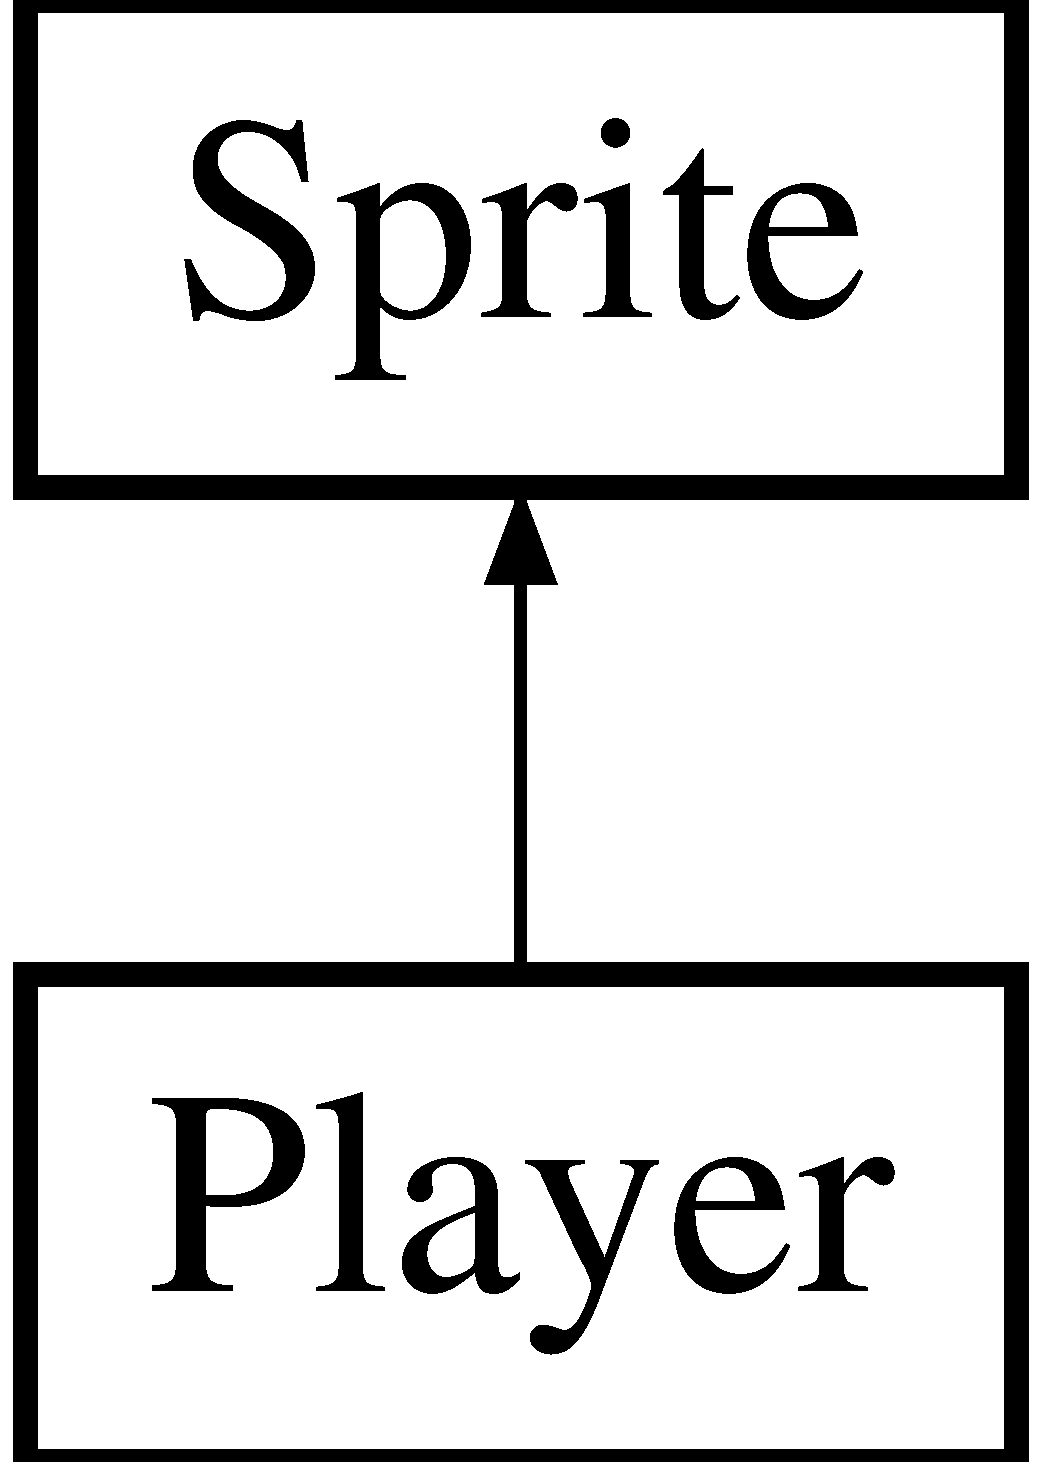
\includegraphics[height=2.000000cm]{classPlayer}
\end{center}
\end{figure}
\subsection*{Public Member Functions}
\begin{DoxyCompactItemize}
\item 
\hyperlink{classPlayer_a2a29c6c2f8635be96415c46c95881954}{Player} (std\-::string \hyperlink{classSprite_aae3514a9a1f77ab5e8e213e44ec618a3}{filename}, short \hyperlink{classSprite_a18eb1c5b90418641d3eabda8f7fe56c9}{x}, short \hyperlink{classSprite_afca2c03aad9d2526427470688ae76439}{y}, unsigned short \hyperlink{classSprite_ac56c9242f797a1a2f76687fca636a3c4}{width}, unsigned short \hyperlink{classSprite_ae96d42c46af7aad1f9031da62f878b21}{height})
\begin{DoxyCompactList}\small\item\em Constructor. \end{DoxyCompactList}\item 
\hyperlink{classPlayer_a749d2c00e1fe0f5c2746f7505a58c062}{$\sim$\-Player} ()
\begin{DoxyCompactList}\small\item\em Destructor. \end{DoxyCompactList}\item 
bool \hyperlink{classPlayer_a83bceadff4531bcd4d8a1112bdd9761c}{touches} (const \hyperlink{classSprite}{Sprite} \&other)
\begin{DoxyCompactList}\small\item\em Check if player touches another \hyperlink{classSprite}{Sprite} class. \end{DoxyCompactList}\item 
void \hyperlink{classPlayer_a27fc37febc547d8d030b24ddae6c10cf}{handle\-Gravity} (const signed S\-C\-R\-E\-E\-N\-\_\-\-W\-I\-D\-T\-H)
\begin{DoxyCompactList}\small\item\em Manages player's movement depending on dx and dy. \end{DoxyCompactList}\item 
void \hyperlink{classPlayer_a1304b1190f969212483e81ae85e86282}{jump} (bool force\-\_\-push=false)
\begin{DoxyCompactList}\small\item\em Jump a short distance into the air. \end{DoxyCompactList}\item 
$\ast$void \hyperlink{classPlayer_ae9c07ea7f8980451fc2070bb5a76f06f}{move} (short dx)
\begin{DoxyCompactList}\small\item\em Set player to in movement on the x-\/axis. \end{DoxyCompactList}\end{DoxyCompactItemize}
\subsection*{Private Attributes}
\begin{DoxyCompactItemize}
\item 
short \hyperlink{classPlayer_a24f9dd9a89dc11513ed416dfaa27743b}{dx\-\_\-}
\item 
short \hyperlink{classPlayer_a744cf17a4642fef56b8fe34abdfe9b74}{dy\-\_\-}
\item 
bool \hyperlink{classPlayer_af64bce8749b5148e518390dea7387ce7}{standing\-\_\-on\-\_\-floor\-\_\-}
\end{DoxyCompactItemize}
\subsection*{Additional Inherited Members}


\subsection{Detailed Description}
\hyperlink{classPlayer}{Player} class. 

\subsection{Constructor \& Destructor Documentation}
\hypertarget{classPlayer_a2a29c6c2f8635be96415c46c95881954}{\index{Player@{Player}!Player@{Player}}
\index{Player@{Player}!Player@{Player}}
\subsubsection[{Player}]{\setlength{\rightskip}{0pt plus 5cm}Player\-::\-Player (
\begin{DoxyParamCaption}
\item[{std\-::string}]{filename, }
\item[{short}]{x, }
\item[{short}]{y, }
\item[{unsigned short}]{width, }
\item[{unsigned short}]{height}
\end{DoxyParamCaption}
)}}\label{classPlayer_a2a29c6c2f8635be96415c46c95881954}


Constructor. 


\begin{DoxyParams}{Parameters}
{\em filename} & Name of object's image-\/file inside graphics/ \\
\hline
{\em x} & starting x-\/position \\
\hline
{\em y} & starting y-\/position \\
\hline
{\em width} & width of image \\
\hline
{\em height} & height of image \\
\hline
\end{DoxyParams}
\hypertarget{classPlayer_a749d2c00e1fe0f5c2746f7505a58c062}{\index{Player@{Player}!$\sim$\-Player@{$\sim$\-Player}}
\index{$\sim$\-Player@{$\sim$\-Player}!Player@{Player}}
\subsubsection[{$\sim$\-Player}]{\setlength{\rightskip}{0pt plus 5cm}Player\-::$\sim$\-Player (
\begin{DoxyParamCaption}
{}
\end{DoxyParamCaption}
)}}\label{classPlayer_a749d2c00e1fe0f5c2746f7505a58c062}


Destructor. 



\subsection{Member Function Documentation}
\hypertarget{classPlayer_a27fc37febc547d8d030b24ddae6c10cf}{\index{Player@{Player}!handle\-Gravity@{handle\-Gravity}}
\index{handle\-Gravity@{handle\-Gravity}!Player@{Player}}
\subsubsection[{handle\-Gravity}]{\setlength{\rightskip}{0pt plus 5cm}void Player\-::handle\-Gravity (
\begin{DoxyParamCaption}
\item[{const signed}]{S\-C\-R\-E\-E\-N\-\_\-\-W\-I\-D\-T\-H}
\end{DoxyParamCaption}
)}}\label{classPlayer_a27fc37febc547d8d030b24ddae6c10cf}


Manages player's movement depending on dx and dy. 


\begin{DoxyParams}{Parameters}
{\em S\-C\-R\-E\-E\-N\-\_\-\-W\-I\-D\-T\-H} & width of game screen \\
\hline
\end{DoxyParams}
\hypertarget{classPlayer_a1304b1190f969212483e81ae85e86282}{\index{Player@{Player}!jump@{jump}}
\index{jump@{jump}!Player@{Player}}
\subsubsection[{jump}]{\setlength{\rightskip}{0pt plus 5cm}void Player\-::jump (
\begin{DoxyParamCaption}
\item[{bool}]{force\-\_\-push = {\ttfamily false}}
\end{DoxyParamCaption}
)}}\label{classPlayer_a1304b1190f969212483e81ae85e86282}


Jump a short distance into the air. 


\begin{DoxyParams}{Parameters}
{\em force\-\_\-push} & if true, this is not due to the player jumping \\
\hline
\end{DoxyParams}
\hypertarget{classPlayer_ae9c07ea7f8980451fc2070bb5a76f06f}{\index{Player@{Player}!move@{move}}
\index{move@{move}!Player@{Player}}
\subsubsection[{move}]{\setlength{\rightskip}{0pt plus 5cm}void Player\-::move (
\begin{DoxyParamCaption}
\item[{short}]{dx}
\end{DoxyParamCaption}
)}}\label{classPlayer_ae9c07ea7f8980451fc2070bb5a76f06f}


Set player to in movement on the x-\/axis. 


\begin{DoxyParams}{Parameters}
{\em dx} & Negative for movement to the left and vice versa \\
\hline
\end{DoxyParams}
\hypertarget{classPlayer_a83bceadff4531bcd4d8a1112bdd9761c}{\index{Player@{Player}!touches@{touches}}
\index{touches@{touches}!Player@{Player}}
\subsubsection[{touches}]{\setlength{\rightskip}{0pt plus 5cm}bool Player\-::touches (
\begin{DoxyParamCaption}
\item[{const {\bf Sprite} \&}]{other}
\end{DoxyParamCaption}
)}}\label{classPlayer_a83bceadff4531bcd4d8a1112bdd9761c}


Check if player touches another \hyperlink{classSprite}{Sprite} class. 


\begin{DoxyParams}{Parameters}
{\em other} & \hyperlink{classSprite}{Sprite} to check if they touch \\
\hline
\end{DoxyParams}
\begin{DoxyReturn}{Returns}
true if they touch 
\end{DoxyReturn}


\subsection{Member Data Documentation}
\hypertarget{classPlayer_a24f9dd9a89dc11513ed416dfaa27743b}{\index{Player@{Player}!dx\-\_\-@{dx\-\_\-}}
\index{dx\-\_\-@{dx\-\_\-}!Player@{Player}}
\subsubsection[{dx\-\_\-}]{\setlength{\rightskip}{0pt plus 5cm}short Player\-::dx\-\_\-\hspace{0.3cm}{\ttfamily [private]}}}\label{classPlayer_a24f9dd9a89dc11513ed416dfaa27743b}
Current x-\/axis movement \hypertarget{classPlayer_a744cf17a4642fef56b8fe34abdfe9b74}{\index{Player@{Player}!dy\-\_\-@{dy\-\_\-}}
\index{dy\-\_\-@{dy\-\_\-}!Player@{Player}}
\subsubsection[{dy\-\_\-}]{\setlength{\rightskip}{0pt plus 5cm}short Player\-::dy\-\_\-\hspace{0.3cm}{\ttfamily [private]}}}\label{classPlayer_a744cf17a4642fef56b8fe34abdfe9b74}
Current y-\/axis movement \hypertarget{classPlayer_af64bce8749b5148e518390dea7387ce7}{\index{Player@{Player}!standing\-\_\-on\-\_\-floor\-\_\-@{standing\-\_\-on\-\_\-floor\-\_\-}}
\index{standing\-\_\-on\-\_\-floor\-\_\-@{standing\-\_\-on\-\_\-floor\-\_\-}!Player@{Player}}
\subsubsection[{standing\-\_\-on\-\_\-floor\-\_\-}]{\setlength{\rightskip}{0pt plus 5cm}bool Player\-::standing\-\_\-on\-\_\-floor\-\_\-\hspace{0.3cm}{\ttfamily [private]}}}\label{classPlayer_af64bce8749b5148e518390dea7387ce7}
True if player has not yet jumped 

The documentation for this class was generated from the following files\-:\begin{DoxyCompactItemize}
\item 
src/\hyperlink{Player_8hh}{Player.\-hh}\item 
src/\hyperlink{Player_8cc}{Player.\-cc}\end{DoxyCompactItemize}

\hypertarget{classSprite}{\section{Sprite Class Reference}
\label{classSprite}\index{Sprite@{Sprite}}
}


Base class for all images.  




{\ttfamily \#include $<$Sprite.\-hh$>$}

Inheritance diagram for Sprite\-:\begin{figure}[H]
\begin{center}
\leavevmode
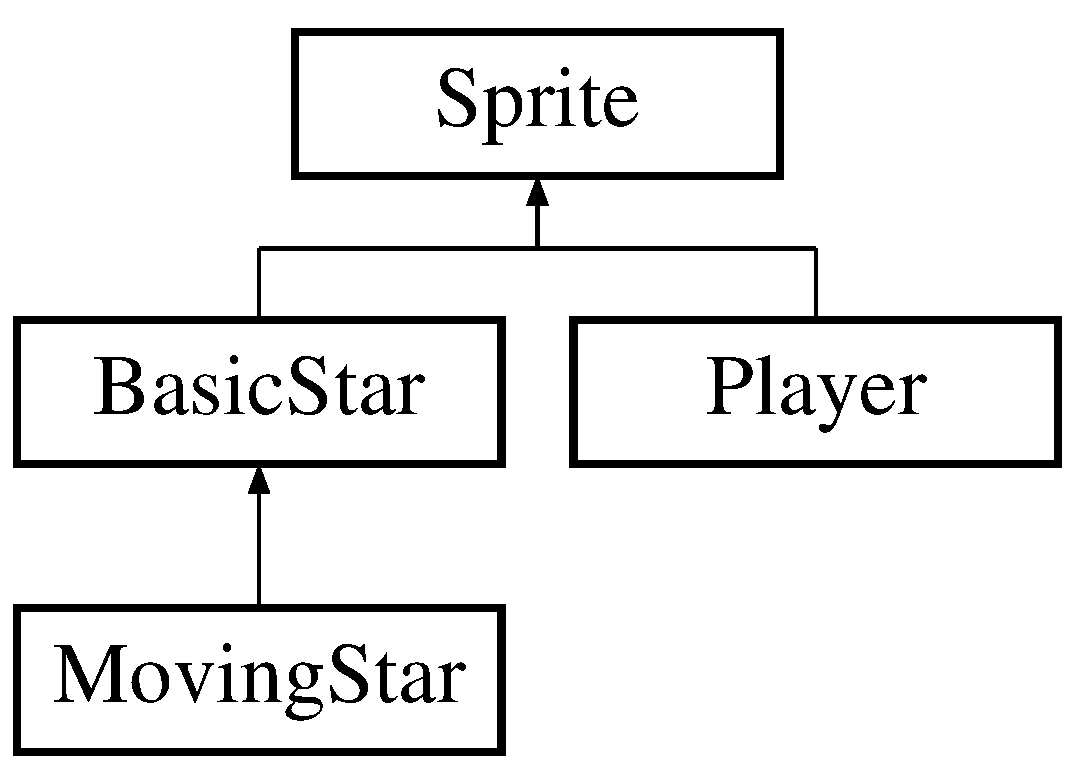
\includegraphics[height=3.000000cm]{classSprite}
\end{center}
\end{figure}
\subsection*{Public Member Functions}
\begin{DoxyCompactItemize}
\item 
\hyperlink{classSprite_a848f031c098042b68984b3840ce64604}{Sprite} (std\-::string \hyperlink{classSprite_aae3514a9a1f77ab5e8e213e44ec618a3}{filename}, short \hyperlink{classSprite_a18eb1c5b90418641d3eabda8f7fe56c9}{x}, short \hyperlink{classSprite_afca2c03aad9d2526427470688ae76439}{y}, unsigned short \hyperlink{classSprite_ac56c9242f797a1a2f76687fca636a3c4}{width}, unsigned short \hyperlink{classSprite_ae96d42c46af7aad1f9031da62f878b21}{height}, short num\-\_\-images)
\begin{DoxyCompactList}\small\item\em Constructor. \end{DoxyCompactList}\item 
\hyperlink{classSprite_ac17f0e18a22c84234a659b1c0bbb69de}{Sprite} (const \hyperlink{classSprite}{Sprite} \&other)
\begin{DoxyCompactList}\small\item\em Copy Constructor. \end{DoxyCompactList}\item 
virtual \hyperlink{classSprite_a8accab430f9d90ae5117b57d67e32b84}{$\sim$\-Sprite} ()
\begin{DoxyCompactList}\small\item\em Destructor. \end{DoxyCompactList}\item 
\hyperlink{classSprite}{Sprite} \& \hyperlink{classSprite_abb3f0673884d42b6b116f0c4d1a47b77}{operator=} (const \hyperlink{classSprite}{Sprite} \&other)
\begin{DoxyCompactList}\small\item\em Copy Constructor. \end{DoxyCompactList}\item 
const std\-::string \& \hyperlink{classSprite_aae3514a9a1f77ab5e8e213e44ec618a3}{filename} () const 
\item 
short \hyperlink{classSprite_a18eb1c5b90418641d3eabda8f7fe56c9}{x} () const 
\item 
short \hyperlink{classSprite_afca2c03aad9d2526427470688ae76439}{y} () const 
\item 
unsigned short \hyperlink{classSprite_ac56c9242f797a1a2f76687fca636a3c4}{width} () const 
\item 
unsigned short \hyperlink{classSprite_ae96d42c46af7aad1f9031da62f878b21}{height} () const 
\item 
virtual short \hyperlink{classSprite_a2703a7a7b2acc1dec83dd1c4f5054aef}{image\-X} ()
\item 
short \hyperlink{classSprite_aa12cd0f64262dcc3c72e0ba2fa39c82d}{initial\-Y} () const 
\begin{DoxyCompactList}\small\item\em the position of the y-\/axis this sprite was initiated at \end{DoxyCompactList}\item 
void \hyperlink{classSprite_a587e5f7d415b1210ffeb091c69818914}{modify\-Y} (int mod)
\begin{DoxyCompactList}\small\item\em Modifies the \hyperlink{classSprite}{Sprite}'s position of the y-\/axis. \end{DoxyCompactList}\end{DoxyCompactItemize}
\subsection*{Protected Attributes}
\begin{DoxyCompactItemize}
\item 
short \hyperlink{classSprite_a8654a8729656ba13695c20c2030de5d0}{current\-\_\-image\-\_\-}
\item 
short \hyperlink{classSprite_a5a6ae065c674bfb85b6d90c1cbfcdca2}{num\-\_\-images\-\_\-}
\item 
short \hyperlink{classSprite_ac66af2df2e5990c07252b8aa0d384346}{x\-\_\-}
\item 
short \hyperlink{classSprite_a3ad6d07d083c5bbb2e819caa31d2bc6f}{y\-\_\-}
\item 
short \hyperlink{classSprite_a2b5cccca24f3c3e0f466624cf034e8a9}{initial\-\_\-y\-\_\-}
\item 
const unsigned short \hyperlink{classSprite_ac0c8b57b52d82f2753c1726e51ed0490}{width\-\_\-}
\item 
const unsigned short \hyperlink{classSprite_ae2ddd489c30852d32b7a88d20af9df1e}{height\-\_\-}
\item 
std\-::string \hyperlink{classSprite_acb2c82f6bea52556153897e9270f219d}{filename\-\_\-}
\end{DoxyCompactItemize}


\subsection{Detailed Description}
Base class for all images. 

\subsection{Constructor \& Destructor Documentation}
\hypertarget{classSprite_a848f031c098042b68984b3840ce64604}{\index{Sprite@{Sprite}!Sprite@{Sprite}}
\index{Sprite@{Sprite}!Sprite@{Sprite}}
\subsubsection[{Sprite}]{\setlength{\rightskip}{0pt plus 5cm}Sprite\-::\-Sprite (
\begin{DoxyParamCaption}
\item[{std\-::string}]{filename, }
\item[{short}]{x, }
\item[{short}]{y, }
\item[{unsigned short}]{width, }
\item[{unsigned short}]{height, }
\item[{short}]{num\-\_\-images}
\end{DoxyParamCaption}
)}}\label{classSprite_a848f031c098042b68984b3840ce64604}


Constructor. 


\begin{DoxyParams}{Parameters}
{\em filename} & Name of the object's image-\/file inside graphics/ \\
\hline
{\em x} & starting x-\/position \\
\hline
{\em y} & starting y-\/position \\
\hline
{\em width} & width of image \\
\hline
{\em height} & height of image \\
\hline
{\em num\-\_\-images} & how many images this \hyperlink{classSprite}{Sprite} has \\
\hline
\end{DoxyParams}
\hypertarget{classSprite_ac17f0e18a22c84234a659b1c0bbb69de}{\index{Sprite@{Sprite}!Sprite@{Sprite}}
\index{Sprite@{Sprite}!Sprite@{Sprite}}
\subsubsection[{Sprite}]{\setlength{\rightskip}{0pt plus 5cm}Sprite\-::\-Sprite (
\begin{DoxyParamCaption}
\item[{const {\bf Sprite} \&}]{other}
\end{DoxyParamCaption}
)}}\label{classSprite_ac17f0e18a22c84234a659b1c0bbb69de}


Copy Constructor. 


\begin{DoxyParams}{Parameters}
{\em other} & \hyperlink{classSprite}{Sprite} to copy \\
\hline
\end{DoxyParams}
\hypertarget{classSprite_a8accab430f9d90ae5117b57d67e32b84}{\index{Sprite@{Sprite}!$\sim$\-Sprite@{$\sim$\-Sprite}}
\index{$\sim$\-Sprite@{$\sim$\-Sprite}!Sprite@{Sprite}}
\subsubsection[{$\sim$\-Sprite}]{\setlength{\rightskip}{0pt plus 5cm}Sprite\-::$\sim$\-Sprite (
\begin{DoxyParamCaption}
{}
\end{DoxyParamCaption}
)\hspace{0.3cm}{\ttfamily [virtual]}}}\label{classSprite_a8accab430f9d90ae5117b57d67e32b84}


Destructor. 



\subsection{Member Function Documentation}
\hypertarget{classSprite_aae3514a9a1f77ab5e8e213e44ec618a3}{\index{Sprite@{Sprite}!filename@{filename}}
\index{filename@{filename}!Sprite@{Sprite}}
\subsubsection[{filename}]{\setlength{\rightskip}{0pt plus 5cm}const std\-::string \& Sprite\-::filename (
\begin{DoxyParamCaption}
{}
\end{DoxyParamCaption}
) const}}\label{classSprite_aae3514a9a1f77ab5e8e213e44ec618a3}
\begin{DoxyReturn}{Returns}
filename of image file 
\end{DoxyReturn}
\hypertarget{classSprite_ae96d42c46af7aad1f9031da62f878b21}{\index{Sprite@{Sprite}!height@{height}}
\index{height@{height}!Sprite@{Sprite}}
\subsubsection[{height}]{\setlength{\rightskip}{0pt plus 5cm}unsigned short Sprite\-::height (
\begin{DoxyParamCaption}
{}
\end{DoxyParamCaption}
) const}}\label{classSprite_ae96d42c46af7aad1f9031da62f878b21}
\begin{DoxyReturn}{Returns}
\hyperlink{classSprite}{Sprite}'s image's height 
\end{DoxyReturn}
\hypertarget{classSprite_a2703a7a7b2acc1dec83dd1c4f5054aef}{\index{Sprite@{Sprite}!image\-X@{image\-X}}
\index{image\-X@{image\-X}!Sprite@{Sprite}}
\subsubsection[{image\-X}]{\setlength{\rightskip}{0pt plus 5cm}short Sprite\-::image\-X (
\begin{DoxyParamCaption}
{}
\end{DoxyParamCaption}
)\hspace{0.3cm}{\ttfamily [virtual]}}}\label{classSprite_a2703a7a7b2acc1dec83dd1c4f5054aef}
\begin{DoxyReturn}{Returns}
x of the image the \hyperlink{classSprite}{Sprite} wants to draw 
\end{DoxyReturn}


Reimplemented in \hyperlink{classPlayer_a41b677053f49c43417ce08dc4f39f62f}{Player}.

\hypertarget{classSprite_aa12cd0f64262dcc3c72e0ba2fa39c82d}{\index{Sprite@{Sprite}!initial\-Y@{initial\-Y}}
\index{initial\-Y@{initial\-Y}!Sprite@{Sprite}}
\subsubsection[{initial\-Y}]{\setlength{\rightskip}{0pt plus 5cm}short Sprite\-::initial\-Y (
\begin{DoxyParamCaption}
{}
\end{DoxyParamCaption}
) const}}\label{classSprite_aa12cd0f64262dcc3c72e0ba2fa39c82d}


the position of the y-\/axis this sprite was initiated at 

\hypertarget{classSprite_a587e5f7d415b1210ffeb091c69818914}{\index{Sprite@{Sprite}!modify\-Y@{modify\-Y}}
\index{modify\-Y@{modify\-Y}!Sprite@{Sprite}}
\subsubsection[{modify\-Y}]{\setlength{\rightskip}{0pt plus 5cm}void Sprite\-::modify\-Y (
\begin{DoxyParamCaption}
\item[{int}]{mod}
\end{DoxyParamCaption}
)}}\label{classSprite_a587e5f7d415b1210ffeb091c69818914}


Modifies the \hyperlink{classSprite}{Sprite}'s position of the y-\/axis. 


\begin{DoxyParams}{Parameters}
{\em mod} & Y axis modifier \\
\hline
\end{DoxyParams}
\hypertarget{classSprite_abb3f0673884d42b6b116f0c4d1a47b77}{\index{Sprite@{Sprite}!operator=@{operator=}}
\index{operator=@{operator=}!Sprite@{Sprite}}
\subsubsection[{operator=}]{\setlength{\rightskip}{0pt plus 5cm}{\bf Sprite} \& Sprite\-::operator= (
\begin{DoxyParamCaption}
\item[{const {\bf Sprite} \&}]{other}
\end{DoxyParamCaption}
)}}\label{classSprite_abb3f0673884d42b6b116f0c4d1a47b77}


Copy Constructor. 


\begin{DoxyParams}{Parameters}
{\em other} & \hyperlink{classSprite}{Sprite} to copy \\
\hline
\end{DoxyParams}
\hypertarget{classSprite_ac56c9242f797a1a2f76687fca636a3c4}{\index{Sprite@{Sprite}!width@{width}}
\index{width@{width}!Sprite@{Sprite}}
\subsubsection[{width}]{\setlength{\rightskip}{0pt plus 5cm}unsigned short Sprite\-::width (
\begin{DoxyParamCaption}
{}
\end{DoxyParamCaption}
) const}}\label{classSprite_ac56c9242f797a1a2f76687fca636a3c4}
\begin{DoxyReturn}{Returns}
\hyperlink{classSprite}{Sprite}'s image's width 
\end{DoxyReturn}
\hypertarget{classSprite_a18eb1c5b90418641d3eabda8f7fe56c9}{\index{Sprite@{Sprite}!x@{x}}
\index{x@{x}!Sprite@{Sprite}}
\subsubsection[{x}]{\setlength{\rightskip}{0pt plus 5cm}short Sprite\-::x (
\begin{DoxyParamCaption}
{}
\end{DoxyParamCaption}
) const}}\label{classSprite_a18eb1c5b90418641d3eabda8f7fe56c9}
\begin{DoxyReturn}{Returns}
\hyperlink{classSprite}{Sprite}'s position of the x-\/axis 
\end{DoxyReturn}
\hypertarget{classSprite_afca2c03aad9d2526427470688ae76439}{\index{Sprite@{Sprite}!y@{y}}
\index{y@{y}!Sprite@{Sprite}}
\subsubsection[{y}]{\setlength{\rightskip}{0pt plus 5cm}short Sprite\-::y (
\begin{DoxyParamCaption}
{}
\end{DoxyParamCaption}
) const}}\label{classSprite_afca2c03aad9d2526427470688ae76439}
\begin{DoxyReturn}{Returns}
\hyperlink{classSprite}{Sprite}'s position of the y-\/axis 
\end{DoxyReturn}


\subsection{Member Data Documentation}
\hypertarget{classSprite_a8654a8729656ba13695c20c2030de5d0}{\index{Sprite@{Sprite}!current\-\_\-image\-\_\-@{current\-\_\-image\-\_\-}}
\index{current\-\_\-image\-\_\-@{current\-\_\-image\-\_\-}!Sprite@{Sprite}}
\subsubsection[{current\-\_\-image\-\_\-}]{\setlength{\rightskip}{0pt plus 5cm}short Sprite\-::current\-\_\-image\-\_\-\hspace{0.3cm}{\ttfamily [protected]}}}\label{classSprite_a8654a8729656ba13695c20c2030de5d0}
If the sprite has many images, this handles them \hypertarget{classSprite_acb2c82f6bea52556153897e9270f219d}{\index{Sprite@{Sprite}!filename\-\_\-@{filename\-\_\-}}
\index{filename\-\_\-@{filename\-\_\-}!Sprite@{Sprite}}
\subsubsection[{filename\-\_\-}]{\setlength{\rightskip}{0pt plus 5cm}std\-::string Sprite\-::filename\-\_\-\hspace{0.3cm}{\ttfamily [protected]}}}\label{classSprite_acb2c82f6bea52556153897e9270f219d}
\hyperlink{classSprite}{Sprite}'s image's filename \hypertarget{classSprite_ae2ddd489c30852d32b7a88d20af9df1e}{\index{Sprite@{Sprite}!height\-\_\-@{height\-\_\-}}
\index{height\-\_\-@{height\-\_\-}!Sprite@{Sprite}}
\subsubsection[{height\-\_\-}]{\setlength{\rightskip}{0pt plus 5cm}const unsigned short Sprite\-::height\-\_\-\hspace{0.3cm}{\ttfamily [protected]}}}\label{classSprite_ae2ddd489c30852d32b7a88d20af9df1e}
\hyperlink{classSprite}{Sprite}'s image's height \hypertarget{classSprite_a2b5cccca24f3c3e0f466624cf034e8a9}{\index{Sprite@{Sprite}!initial\-\_\-y\-\_\-@{initial\-\_\-y\-\_\-}}
\index{initial\-\_\-y\-\_\-@{initial\-\_\-y\-\_\-}!Sprite@{Sprite}}
\subsubsection[{initial\-\_\-y\-\_\-}]{\setlength{\rightskip}{0pt plus 5cm}short Sprite\-::initial\-\_\-y\-\_\-\hspace{0.3cm}{\ttfamily [protected]}}}\label{classSprite_a2b5cccca24f3c3e0f466624cf034e8a9}
\hypertarget{classSprite_a5a6ae065c674bfb85b6d90c1cbfcdca2}{\index{Sprite@{Sprite}!num\-\_\-images\-\_\-@{num\-\_\-images\-\_\-}}
\index{num\-\_\-images\-\_\-@{num\-\_\-images\-\_\-}!Sprite@{Sprite}}
\subsubsection[{num\-\_\-images\-\_\-}]{\setlength{\rightskip}{0pt plus 5cm}short Sprite\-::num\-\_\-images\-\_\-\hspace{0.3cm}{\ttfamily [protected]}}}\label{classSprite_a5a6ae065c674bfb85b6d90c1cbfcdca2}
How many images a \hyperlink{classSprite}{Sprite} has \hypertarget{classSprite_ac0c8b57b52d82f2753c1726e51ed0490}{\index{Sprite@{Sprite}!width\-\_\-@{width\-\_\-}}
\index{width\-\_\-@{width\-\_\-}!Sprite@{Sprite}}
\subsubsection[{width\-\_\-}]{\setlength{\rightskip}{0pt plus 5cm}const unsigned short Sprite\-::width\-\_\-\hspace{0.3cm}{\ttfamily [protected]}}}\label{classSprite_ac0c8b57b52d82f2753c1726e51ed0490}
\hyperlink{classSprite}{Sprite}'s original position on the y-\/axis \hyperlink{classSprite}{Sprite}'s image's width \hypertarget{classSprite_ac66af2df2e5990c07252b8aa0d384346}{\index{Sprite@{Sprite}!x\-\_\-@{x\-\_\-}}
\index{x\-\_\-@{x\-\_\-}!Sprite@{Sprite}}
\subsubsection[{x\-\_\-}]{\setlength{\rightskip}{0pt plus 5cm}short Sprite\-::x\-\_\-\hspace{0.3cm}{\ttfamily [protected]}}}\label{classSprite_ac66af2df2e5990c07252b8aa0d384346}
\hyperlink{classSprite}{Sprite}'s position on the x-\/axis \hypertarget{classSprite_a3ad6d07d083c5bbb2e819caa31d2bc6f}{\index{Sprite@{Sprite}!y\-\_\-@{y\-\_\-}}
\index{y\-\_\-@{y\-\_\-}!Sprite@{Sprite}}
\subsubsection[{y\-\_\-}]{\setlength{\rightskip}{0pt plus 5cm}short Sprite\-::y\-\_\-\hspace{0.3cm}{\ttfamily [protected]}}}\label{classSprite_a3ad6d07d083c5bbb2e819caa31d2bc6f}
\hyperlink{classSprite}{Sprite}'s position on the y-\/acis 

The documentation for this class was generated from the following files\-:\begin{DoxyCompactItemize}
\item 
src/\hyperlink{Sprite_8hh}{Sprite.\-hh}\item 
src/\hyperlink{Sprite_8cc}{Sprite.\-cc}\end{DoxyCompactItemize}

\chapter{File Documentation}
\hypertarget{BasicStar_8cc}{\section{src/\-Basic\-Star.cc File Reference}
\label{BasicStar_8cc}\index{src/\-Basic\-Star.\-cc@{src/\-Basic\-Star.\-cc}}
}
{\ttfamily \#include $<$random$>$}\\*
{\ttfamily \#include $<$chrono$>$}\\*
{\ttfamily \#include \char`\"{}Basic\-Star.\-hh\char`\"{}}\\*

\hypertarget{BasicStar_8hh}{\section{src/\-Basic\-Star.hh File Reference}
\label{BasicStar_8hh}\index{src/\-Basic\-Star.\-hh@{src/\-Basic\-Star.\-hh}}
}


File containing the \hyperlink{classBasicStar}{Basic\-Star} class Header.  


{\ttfamily \#include \char`\"{}Sprite.\-hh\char`\"{}}\\*
\subsection*{Classes}
\begin{DoxyCompactItemize}
\item 
class \hyperlink{classBasicStar}{Basic\-Star}
\begin{DoxyCompactList}\small\item\em The most basic type of star, cannot move. \end{DoxyCompactList}\end{DoxyCompactItemize}


\subsection{Detailed Description}
File containing the \hyperlink{classBasicStar}{Basic\-Star} class Header. \begin{DoxyAuthor}{Author}
Olle Kvarnström 
\end{DoxyAuthor}
\begin{DoxyDate}{Date}

\end{DoxyDate}

\hypertarget{Game_8cc}{\section{src/\-Game.cc File Reference}
\label{Game_8cc}\index{src/\-Game.\-cc@{src/\-Game.\-cc}}
}
{\ttfamily \#include $<$iostream$>$}\\*
{\ttfamily \#include $<$string$>$}\\*
{\ttfamily \#include $<$algorithm$>$}\\*
{\ttfamily \#include \char`\"{}Game.\-hh\char`\"{}}\\*

\hypertarget{Game_8hh}{\section{src/\-Game.hh File Reference}
\label{Game_8hh}\index{src/\-Game.\-hh@{src/\-Game.\-hh}}
}


File containing the \hyperlink{classGame}{Game} class Header.  


{\ttfamily \#include $<$list$>$}\\*
{\ttfamily \#include \char`\"{}Graphics\-Engine.\-hh\char`\"{}}\\*
{\ttfamily \#include \char`\"{}Sprite.\-hh\char`\"{}}\\*
{\ttfamily \#include \char`\"{}Player.\-hh\char`\"{}}\\*
{\ttfamily \#include \char`\"{}Basic\-Enemy.\-hh\char`\"{}}\\*
\subsection*{Classes}
\begin{DoxyCompactItemize}
\item 
class \hyperlink{classGame}{Game}
\begin{DoxyCompactList}\small\item\em Main game class. \end{DoxyCompactList}\end{DoxyCompactItemize}


\subsection{Detailed Description}
File containing the \hyperlink{classGame}{Game} class Header. \begin{DoxyAuthor}{Author}
Olle Kvarnström 
\end{DoxyAuthor}
\begin{DoxyDate}{Date}

\end{DoxyDate}

\hypertarget{GraphicsEngine_8cc}{\section{src/\-Graphics\-Engine.cc File Reference}
\label{GraphicsEngine_8cc}\index{src/\-Graphics\-Engine.\-cc@{src/\-Graphics\-Engine.\-cc}}
}
{\ttfamily \#include \char`\"{}Graphics\-Engine.\-hh\char`\"{}}\\*
{\ttfamily \#include $<$iostream$>$}\\*
{\ttfamily \#include $<$algorithm$>$}\\*

\hypertarget{GraphicsEngine_8hh}{\section{src/\-Graphics\-Engine.hh File Reference}
\label{GraphicsEngine_8hh}\index{src/\-Graphics\-Engine.\-hh@{src/\-Graphics\-Engine.\-hh}}
}


File containing the \hyperlink{classGraphicsEngine}{Graphics\-Engine} class Header.  


{\ttfamily \#include $<$string$>$}\\*
{\ttfamily \#include $<$map$>$}\\*
{\ttfamily \#include $<$S\-D\-L/\-S\-D\-L.\-h$>$}\\*
{\ttfamily \#include $<$S\-D\-L/\-S\-D\-L\-\_\-image.\-h$>$}\\*
\subsection*{Classes}
\begin{DoxyCompactItemize}
\item 
class \hyperlink{classGraphicsEngine}{Graphics\-Engine}
\begin{DoxyCompactList}\small\item\em Class for managing graphics and events. \end{DoxyCompactList}\end{DoxyCompactItemize}
\subsection*{Typedefs}
\begin{DoxyCompactItemize}
\item 
typedef S\-D\-L\-\_\-\-Rect \hyperlink{GraphicsEngine_8hh_a9a150f1ad43ec7de65cfe698cdae8bee}{rect\-\_\-t}
\end{DoxyCompactItemize}
\subsection*{Enumerations}
\begin{DoxyCompactItemize}
\item 
enum \hyperlink{GraphicsEngine_8hh_a2fb9b58e4e5f14f40af8b4a1425841f8}{event\-\_\-t} \{ \\*
\hyperlink{GraphicsEngine_8hh_a2fb9b58e4e5f14f40af8b4a1425841f8adb45120aafd37a973140edee24708065}{L\-E\-F\-T}, 
\hyperlink{GraphicsEngine_8hh_a2fb9b58e4e5f14f40af8b4a1425841f8aec8379af7490bb9eaaf579cf17876f38}{R\-I\-G\-H\-T}, 
\hyperlink{GraphicsEngine_8hh_a2fb9b58e4e5f14f40af8b4a1425841f8aba595d8bca8bc5e67c37c0a9d89becfa}{U\-P}, 
\hyperlink{GraphicsEngine_8hh_a2fb9b58e4e5f14f40af8b4a1425841f8af63c0ddcabcef7eafa6b68908ffce431}{S\-T\-I\-L\-L}, 
\\*
\hyperlink{GraphicsEngine_8hh_a2fb9b58e4e5f14f40af8b4a1425841f8acfe24a7b308a82835c8a9a9a89bc4ca2}{N\-O\-T\-H\-I\-N\-G}, 
\hyperlink{GraphicsEngine_8hh_a2fb9b58e4e5f14f40af8b4a1425841f8a76bdc8adfd6c6463ab269ff4c06be9b4}{Q\-U\-I\-T}
 \}
\begin{DoxyCompactList}\small\item\em events describing user input \end{DoxyCompactList}\end{DoxyCompactItemize}


\subsection{Detailed Description}
File containing the \hyperlink{classGraphicsEngine}{Graphics\-Engine} class Header. \begin{DoxyAuthor}{Author}
Olle Kvarnström 
\end{DoxyAuthor}
\begin{DoxyDate}{Date}

\end{DoxyDate}


\subsection{Typedef Documentation}
\hypertarget{GraphicsEngine_8hh_a9a150f1ad43ec7de65cfe698cdae8bee}{\index{Graphics\-Engine.\-hh@{Graphics\-Engine.\-hh}!rect\-\_\-t@{rect\-\_\-t}}
\index{rect\-\_\-t@{rect\-\_\-t}!GraphicsEngine.hh@{Graphics\-Engine.\-hh}}
\subsubsection[{rect\-\_\-t}]{\setlength{\rightskip}{0pt plus 5cm}typedef S\-D\-L\-\_\-\-Rect {\bf rect\-\_\-t}}}\label{GraphicsEngine_8hh_a9a150f1ad43ec7de65cfe698cdae8bee}


\subsection{Enumeration Type Documentation}
\hypertarget{GraphicsEngine_8hh_a2fb9b58e4e5f14f40af8b4a1425841f8}{\index{Graphics\-Engine.\-hh@{Graphics\-Engine.\-hh}!event\-\_\-t@{event\-\_\-t}}
\index{event\-\_\-t@{event\-\_\-t}!GraphicsEngine.hh@{Graphics\-Engine.\-hh}}
\subsubsection[{event\-\_\-t}]{\setlength{\rightskip}{0pt plus 5cm}enum {\bf event\-\_\-t}}}\label{GraphicsEngine_8hh_a2fb9b58e4e5f14f40af8b4a1425841f8}


events describing user input 

\begin{Desc}
\item[Enumerator]\par
\begin{description}
\index{L\-E\-F\-T@{L\-E\-F\-T}!Graphics\-Engine.\-hh@{Graphics\-Engine.\-hh}}\index{Graphics\-Engine.\-hh@{Graphics\-Engine.\-hh}!L\-E\-F\-T@{L\-E\-F\-T}}\item[{\em 
\hypertarget{GraphicsEngine_8hh_a2fb9b58e4e5f14f40af8b4a1425841f8adb45120aafd37a973140edee24708065}{L\-E\-F\-T}\label{GraphicsEngine_8hh_a2fb9b58e4e5f14f40af8b4a1425841f8adb45120aafd37a973140edee24708065}
}]\hyperlink{classPlayer}{Player} wants to move left \index{R\-I\-G\-H\-T@{R\-I\-G\-H\-T}!Graphics\-Engine.\-hh@{Graphics\-Engine.\-hh}}\index{Graphics\-Engine.\-hh@{Graphics\-Engine.\-hh}!R\-I\-G\-H\-T@{R\-I\-G\-H\-T}}\item[{\em 
\hypertarget{GraphicsEngine_8hh_a2fb9b58e4e5f14f40af8b4a1425841f8aec8379af7490bb9eaaf579cf17876f38}{R\-I\-G\-H\-T}\label{GraphicsEngine_8hh_a2fb9b58e4e5f14f40af8b4a1425841f8aec8379af7490bb9eaaf579cf17876f38}
}]\hyperlink{classPlayer}{Player} wants to move right \index{U\-P@{U\-P}!Graphics\-Engine.\-hh@{Graphics\-Engine.\-hh}}\index{Graphics\-Engine.\-hh@{Graphics\-Engine.\-hh}!U\-P@{U\-P}}\item[{\em 
\hypertarget{GraphicsEngine_8hh_a2fb9b58e4e5f14f40af8b4a1425841f8aba595d8bca8bc5e67c37c0a9d89becfa}{U\-P}\label{GraphicsEngine_8hh_a2fb9b58e4e5f14f40af8b4a1425841f8aba595d8bca8bc5e67c37c0a9d89becfa}
}]\hyperlink{classPlayer}{Player} wants to jump \index{S\-T\-I\-L\-L@{S\-T\-I\-L\-L}!Graphics\-Engine.\-hh@{Graphics\-Engine.\-hh}}\index{Graphics\-Engine.\-hh@{Graphics\-Engine.\-hh}!S\-T\-I\-L\-L@{S\-T\-I\-L\-L}}\item[{\em 
\hypertarget{GraphicsEngine_8hh_a2fb9b58e4e5f14f40af8b4a1425841f8af63c0ddcabcef7eafa6b68908ffce431}{S\-T\-I\-L\-L}\label{GraphicsEngine_8hh_a2fb9b58e4e5f14f40af8b4a1425841f8af63c0ddcabcef7eafa6b68908ffce431}
}]\hyperlink{classPlayer}{Player} wants to stop moving \index{N\-O\-T\-H\-I\-N\-G@{N\-O\-T\-H\-I\-N\-G}!Graphics\-Engine.\-hh@{Graphics\-Engine.\-hh}}\index{Graphics\-Engine.\-hh@{Graphics\-Engine.\-hh}!N\-O\-T\-H\-I\-N\-G@{N\-O\-T\-H\-I\-N\-G}}\item[{\em 
\hypertarget{GraphicsEngine_8hh_a2fb9b58e4e5f14f40af8b4a1425841f8acfe24a7b308a82835c8a9a9a89bc4ca2}{N\-O\-T\-H\-I\-N\-G}\label{GraphicsEngine_8hh_a2fb9b58e4e5f14f40af8b4a1425841f8acfe24a7b308a82835c8a9a9a89bc4ca2}
}]Unknown input received \index{Q\-U\-I\-T@{Q\-U\-I\-T}!Graphics\-Engine.\-hh@{Graphics\-Engine.\-hh}}\index{Graphics\-Engine.\-hh@{Graphics\-Engine.\-hh}!Q\-U\-I\-T@{Q\-U\-I\-T}}\item[{\em 
\hypertarget{GraphicsEngine_8hh_a2fb9b58e4e5f14f40af8b4a1425841f8a76bdc8adfd6c6463ab269ff4c06be9b4}{Q\-U\-I\-T}\label{GraphicsEngine_8hh_a2fb9b58e4e5f14f40af8b4a1425841f8a76bdc8adfd6c6463ab269ff4c06be9b4}
}]User wants to exit the game \end{description}
\end{Desc}

\hypertarget{main_8cc}{\section{src/main.cc File Reference}
\label{main_8cc}\index{src/main.\-cc@{src/main.\-cc}}
}
{\ttfamily \#include \char`\"{}Game.\-hh\char`\"{}}\\*
\subsection*{Functions}
\begin{DoxyCompactItemize}
\item 
int \hyperlink{main_8cc_ae66f6b31b5ad750f1fe042a706a4e3d4}{main} ()
\end{DoxyCompactItemize}


\subsection{Function Documentation}
\hypertarget{main_8cc_ae66f6b31b5ad750f1fe042a706a4e3d4}{\index{main.\-cc@{main.\-cc}!main@{main}}
\index{main@{main}!main.cc@{main.\-cc}}
\subsubsection[{main}]{\setlength{\rightskip}{0pt plus 5cm}int main (
\begin{DoxyParamCaption}
{}
\end{DoxyParamCaption}
)}}\label{main_8cc_ae66f6b31b5ad750f1fe042a706a4e3d4}

\hypertarget{Player_8cc}{\section{src/\-Player.cc File Reference}
\label{Player_8cc}\index{src/\-Player.\-cc@{src/\-Player.\-cc}}
}
{\ttfamily \#include $<$cmath$>$}\\*
{\ttfamily \#include \char`\"{}Player.\-hh\char`\"{}}\\*

\hypertarget{Player_8hh}{\section{src/\-Player.hh File Reference}
\label{Player_8hh}\index{src/\-Player.\-hh@{src/\-Player.\-hh}}
}


File containing the \hyperlink{classPlayer}{Player} class Header.  


{\ttfamily \#include \char`\"{}Sprite.\-hh\char`\"{}}\\*
\subsection*{Classes}
\begin{DoxyCompactItemize}
\item 
class \hyperlink{classPlayer}{Player}
\begin{DoxyCompactList}\small\item\em \hyperlink{classPlayer}{Player} class. \end{DoxyCompactList}\end{DoxyCompactItemize}


\subsection{Detailed Description}
File containing the \hyperlink{classPlayer}{Player} class Header. \begin{DoxyAuthor}{Author}
Olle Kvarnström 
\end{DoxyAuthor}
\begin{DoxyDate}{Date}

\end{DoxyDate}

\hypertarget{Sprite_8cc}{\section{src/\-Sprite.cc File Reference}
\label{Sprite_8cc}\index{src/\-Sprite.\-cc@{src/\-Sprite.\-cc}}
}
{\ttfamily \#include \char`\"{}Sprite.\-hh\char`\"{}}\\*

\hypertarget{Sprite_8hh}{\section{src/\-Sprite.hh File Reference}
\label{Sprite_8hh}\index{src/\-Sprite.\-hh@{src/\-Sprite.\-hh}}
}


File containing the \hyperlink{classSprite}{Sprite} class Header.  


{\ttfamily \#include $<$string$>$}\\*
\subsection*{Classes}
\begin{DoxyCompactItemize}
\item 
class \hyperlink{classSprite}{Sprite}
\begin{DoxyCompactList}\small\item\em Base class for all images. \end{DoxyCompactList}\end{DoxyCompactItemize}


\subsection{Detailed Description}
File containing the \hyperlink{classSprite}{Sprite} class Header. \begin{DoxyAuthor}{Author}
Olle Kvarnström 
\end{DoxyAuthor}
\begin{DoxyDate}{Date}

\end{DoxyDate}

%--- End generated contents ---

% Index
\newpage
\phantomsection
\addcontentsline{toc}{part}{Index}
\printindex

\end{document}
